% ============================================================================
% MÉMOIRE v2 — Allocation de capital sous contraintes réglementaires
% Document maître : compiler ce fichier uniquement.
% ============================================================================
\documentclass[10pt, a4paper, oneside]{report}

% ─── Encodage & langue ────────────────────────────────────
\usepackage[utf8]{inputenc}
\usepackage[T1]{fontenc}
\usepackage[authoryear, round]{natbib}
\usepackage[french]{babel}
\usepackage{csquotes}

% ─── Police ───────────────────────────────────────────────
\usepackage{mathpazo}          % Palatino (serif, lisible, académique)
\usepackage[scaled=0.85]{helvet}
\usepackage{microtype}         % Améliorations typographiques fines
\emergencystretch=2em          % Palatino 10pt : éviter les overfull hbox

% ─── Couleurs ────────────────────────────────────────────
\usepackage{xcolor}
\definecolor{bleutitre}{RGB}{0, 51, 102}     % bleu marine sobre
\definecolor{bleulien}{RGB}{0, 70, 130}      % bleu légèrement plus clair

% ─── Géométrie ────────────────────────────────────────────
\usepackage{geometry}
\geometry{
  top=2.5cm,
  bottom=2.5cm,
  left=3cm,
  right=2.5cm,
  headheight=15pt,
}
\usepackage{setspace}
\onehalfspacing

% ─── Mathématiques ────────────────────────────────────────
\usepackage{amsmath, amssymb, amsthm}
\usepackage{mathtools}

% ─── Tableaux & listes ───────────────────────────────────
\usepackage{booktabs}
\usepackage{multirow}
\usepackage{array}
\usepackage{longtable}
\usepackage{enumitem}
\usepackage{textcomp}
\usepackage{ragged2e}
\usepackage{hyphenat}
\usepackage[most]{tcolorbox}

% ─── Graphiques ───────────────────────────────────────────
\usepackage{graphicx}
\usepackage{tikz}
\usetikzlibrary{positioning}
\usepackage{caption}
\usepackage{subcaption}

% ─── Algorithmes ──────────────────────────────────────────
\usepackage{algorithm}
\usepackage{algpseudocode}

% ─── En-têtes et pieds de page ────────────────────────────
\usepackage{fancyhdr}
\pagestyle{fancy}
\fancyhf{}
\fancyhead[L]{\small\itshape\nouppercase{\leftmark}}
\fancyhead[R]{}
\fancyfoot[C]{\thepage}
\renewcommand{\headrulewidth}{0.4pt}

\fancypagestyle{plain}{%
  \fancyhf{}
  \fancyfoot[C]{\thepage}
  \renewcommand{\headrulewidth}{0pt}
}

% ─── Liens ────────────────────────────────────────────────
\usepackage{hyperref}
\hypersetup{
  colorlinks=true,
  linkcolor=bleutitre,
  citecolor=bleulien,
  urlcolor=bleulien,
  pdftitle={Allocation de capital sous contraintes réglementaires},
  pdfauthor={},
}

% ─── Bibliographie ────────────────────────────────────────
% natbib chargé avant babel (cf. french3.ldf warning)

% ─── Titres colorés ─────────────────────────────────────
\usepackage{titlesec}
\titleformat{\chapter}[display]
  {\bfseries\Large\color{bleutitre}}{\chaptertitlename~\thechapter}{15pt}{\LARGE}
\titleformat{\section}
  {\bfseries\large\color{bleutitre}}{\thesection}{1em}{}
\titleformat{\subsection}
  {\bfseries\normalsize\color{bleutitre}}{\thesubsection}{1em}{}

% ─── Théorèmes & définitions ─────────────────────────────
\theoremstyle{definition}
\newtheorem{definition}{Définition}[chapter]
\newtheorem{proposition}{Proposition}[chapter]
\newtheorem{remarque}{Remarque}[chapter]

% ============================================================================
\begin{document}

% ── Page de titre ─────────────────────────────────────────
\begin{titlepage}
\centering
\vspace*{3cm}

{\Huge\bfseries Allocation de capital\\[0.4em]
sous contraintes réglementaires}

\vspace{1.5cm}

{\LARGE IFRS~9, IFRS~13, Bâle~III\,/\,CRR3}

\vspace{3cm}

\rule{0.5\textwidth}{0.5pt}

\vspace{2cm}

{\Large Mémoire}

\vspace{1.5cm}

{\large
\textbf{Domaine~:} Gestion des risques financiers\\[0.5em]
\textbf{Méthode~:} Data science et optimisation sous contraintes
}

\vfill

{\large 2026}

\end{titlepage}
\thispagestyle{empty}

% ── Table des matières ────────────────────────────────────
\tableofcontents
\newpage


% ══════════════════════════════════════════════════════════
% INTRODUCTION
% ══════════════════════════════════════════════════════════

\chapter*{Introduction}
\addcontentsline{toc}{chapter}{Introduction}
\markboth{Introduction}{Introduction}
\label{chap:introduction}

% ── MOVE 1 : Établir le territoire ─────────────────────────

La crise financière de 2008 a révélé que les banques pouvaient détenir des portefeuilles individuellement acceptables mais collectivement fragiles.
En réponse, le législateur a profondément remanié le cadre normatif~: IFRS~9 \citep{ifrs9} a remplacé le provisionnement rétrospectif d'IAS~39 (l'ancienne norme, qui ne constituait une provision qu'après la constatation d'une perte) par un modèle prospectif en trois stades~; CRR3 \citep{crr3} a durci les pondérations de risque, en particulier sur les expositions en actions et en private equity~; Bâle~III \citep{bcbs_d424} a introduit des ratios de liquidité (LCR, NSFR) et un encadrement du risque de taux (IRRBB).
Ces réformes ont rendu le bilan bancaire plus résilient, mais aussi plus contraint~: chaque classe d'actifs obéit désormais à un corpus réglementaire propre, et l'allocation du capital entre elles est devenue un problème d'optimisation sous contraintes multiples.

La littérature sur l'allocation de capital bancaire est abondante mais fragmentée.
Les travaux fondateurs de \citet{merton1974} et \citet{vasicek2002} ont posé les bases de la modélisation du risque de crédit en portefeuille, prolongées par \citet{gordy2003} dans le cadre du modèle ASRF (\emph{Asymptotic Single Risk Factor}~: tous les emprunteurs partagent un unique facteur de risque systématique), qui sous-tend les exigences de capital de Bâle~II et~III.
L'estimation des paramètres de risque (PD, LGD, EAD) a fait l'objet d'un cadre réglementaire détaillé \citep{eba_gl_2017_06, eba_gl_2019_03} et d'une littérature appliquée sur les modèles de scoring \citep{siddiqi2006, hosmer_lemeshow2013}.
Plus récemment, les méthodes d'apprentissage automatique --- TabNet \citep{arik_pfister2021}, XGBoost \citep{chen_guestrin2016} --- ont démontré leur capacité à capturer des non-linéarités que les modèles traditionnels ignorent \citep{grinsztajn2022}.

Du côté de l'optimisation de portefeuille, le modèle de \citet{black_litterman1992} permet de combiner un équilibre de marché avec des vues subjectives, tandis que la CVaR (\emph{Conditional Value-at-Risk}~: la perte moyenne au-delà d'un seuil de confiance, ici le 95\textsuperscript{e} percentile) \citep{rockafellar_uryasev2000} offre une mesure de risque cohérente adaptée aux distributions à queue épaisse.
L'allocation de capital au sein d'une banque a été formalisée par \citet{tasche2008} via le principe d'Euler, et le cadre général du risque quantitatif est couvert par \citet{mcneil_frey_embrechts2015}.

Enfin, la valorisation du private equity en juste valeur (IFRS~13) fait l'objet de guidelines spécifiques \citep{ipev2022}, et les données de marché --- décotes de liquidité \citep{jefferies_lazard2023}, performance par vintage \citep{cambridge2023}, taux de défaut par notation \citep{moodys_default2023} --- permettent de calibrer les modèles.

% ── MOVE 2 : Établir la niche (gap) ────────────────────────

Toutefois, ces travaux abordent chaque dimension du problème de manière isolée.
Les modèles de risque de crédit ne traitent pas de la valorisation PE.
Les méthodes d'optimisation de portefeuille ne modélisent pas le staging IFRS~9.
Les guidelines de provisionnement n'intègrent pas les contraintes de liquidité.
En pratique, le provisionnement crédit, la valorisation PE, l'optimisation du capital et le suivi de la liquidité sont réalisés par des équipes distinctes, avec des outils distincts, et remontent au comité des risques comme des rapports séparés.

Il n'existe pas, à notre connaissance, de cadre intégré qui permette d'optimiser l'allocation du capital d'une banque sous l'ensemble des contraintes réglementaires --- IFRS~9, IFRS~13, CRR3, LCR, NSFR, IRRBB --- en modélisant conjointement toutes les classes d'actifs face aux mêmes chocs macroéconomiques.

% ── MOVE 3 : Occuper la niche ──────────────────────────────

Ce mémoire se propose de combler cette lacune en répondant à la question suivante~:

\medskip
\begin{quote}
\itshape
Sous les contraintes conjointes d'IFRS~9, d'IFRS~13 et de Bâle~III, quelle est l'allocation optimale du capital d'un établissement financier entre ses classes d'actifs~?
\end{quote}
\medskip

Pour y répondre, nous construisons un cadre d'analyse intégré et l'appliquons à deux échelles successives.
Ce travail apporte quatre contributions~:

\begin{enumerate}
  \item \textbf{Un cadre unifié multi-normes.}
  Nous proposons un pipeline qui modélise conjointement le provisionnement IFRS~9, la valorisation IFRS~13, la consommation de capital CRR3, et les ratios de liquidité (LCR, NSFR), alimenté par les mêmes variables macroéconomiques et testé sur douze scénarios historiquement calibrés.

  \item \textbf{Des résultats sur la nature de l'arbitrage.}
  En partant du cas crédit contre PE --- deux classes aux profils de risque opposés --- puis en étendant l'analyse à quatorze classes d'actifs via un optimiseur Black-Litterman CVaR, nous identifions où se situe réellement le levier d'allocation.

  \item \textbf{Un résultat de sensibilité sur les déterminants de l'allocation.}
  L'analyse systématique de 384 configurations de modélisation montre que, dans le cadre calibré, un paramètre rarement discuté dans la littérature a un impact de premier ordre sur l'allocation --- plus que l'algorithme d'optimisation lui-même.

  \item \textbf{Un outillage complet.}
  Un pipeline intégré --- du générateur de données synthétiques au tableau de bord CRO --- incluant trois familles de modèles PD, un optimiseur multi-contraintes, et un dashboard interactif. Le pipeline est reproductible via graines fixes et validé par $\sim$700 tests unitaires.
\end{enumerate}

L'approche repose sur des données synthétiques calibrées sur des sources institutionnelles (EBA, Moody's, Cambridge Associates), trois familles de modèles de probabilité de défaut (régression logistique, TabNet, XGBoost), et un optimiseur multi-contraintes.
Le tout est intégré dans un tableau de bord interactif destiné au directeur des risques.

La figure~\ref{fig:pipeline} résume l'architecture du pipeline intégré.

\begin{figure}[htbp]
\centering
\begin{tikzpicture}[
  node distance=0.6cm and 0.9cm,
  block/.style={rectangle, draw=bleutitre, fill=bleutitre!8, text width=2.4cm, text centered, rounded corners, minimum height=0.85cm, font=\small},
  arrow/.style={->, >=stealth, thick, color=bleutitre!70}
]
% Row 1
\node[block] (dgp) {\textbf{DGP}\\[-2pt]{\scriptsize 30\,000 clients}};
\node[block, right=of dgp] (pd) {\textbf{Modèles PD}\\[-2pt]{\scriptsize LR, TabNet, XGB}};
\node[block, right=of pd] (ecl) {\textbf{Moteur ECL}\\[-2pt]{\scriptsize SICR $\cdot$ LGD $\cdot$ EAD}};
\node[block, right=of ecl] (met) {\textbf{Métriques}\\[-2pt]{\scriptsize RAROC, EVA}};
% Row 2
\node[block, below=of met] (opt) {\textbf{Optimiseur}\\[-2pt]{\scriptsize BL-CVaR}};
\node[block, left=of opt] (dash) {\textbf{Dashboard}\\[-2pt]{\scriptsize CRO interactif}};
% Arrows
\draw[arrow] (dgp) -- (pd);
\draw[arrow] (pd) -- (ecl);
\draw[arrow] (ecl) -- (met);
\draw[arrow] (met) -- (opt);
\draw[arrow] (opt) -- (dash);
\end{tikzpicture}
\caption{Architecture du pipeline intégré~: du processus générateur de données au tableau de bord CRO.}
\label{fig:pipeline}
\end{figure}

Le mémoire est organisé en quatre chapitres. Le premier construit le pipeline complet --- du portefeuille synthétique aux métriques de décision --- et quantifie l'arbitrage crédit/PE sur cinq secteurs. Le deuxième étend l'analyse à quatorze classes d'actifs et présente l'optimiseur BL-CVaR. Le troisième analyse l'allocation résultante et quantifie le coût de la franchise bancaire. Le quatrième évalue le risque de spécification du facteur systématique.


% ══════════════════════════════════════════════════════════
% CHAPITRE 1 — Données, modèles et moteur de pertes
% ══════════════════════════════════════════════════════════

\chapter{Le cadre intégré}
\label{chap:cadre}

Ce chapitre construit le pipeline complet~: portefeuille synthétique, modèles de scoring, moteur de pertes IFRS~9, métriques de décision (RAROC, EVA), et valorisation du private equity. Il quantifie l'arbitrage crédit/PE sur cinq secteurs avant de poser la question de l'échelle.


\section{Le portefeuille synthétique}
\label{sec:ch1:dgp}

Le recours à des données synthétiques est un choix méthodologique délibéré, motivé par trois raisons. Premièrement, les données bancaires réelles sont confidentielles~: aucun portefeuille de crédit d'une banque européenne n'est librement disponible à la granularité nécessaire (30\,000 contreparties, 15 variables financières, historique de retard de paiement). Deuxièmement, un processus générateur de données (DGP) contrôlé permet de connaître \emph{exactement} les relations entre variables et défaut, ce qui autorise un diagnostic précis des forces et faiblesses de chaque modèle de scoring --- une propriété impossible avec des données réelles où le vrai DGP est inconnu. Troisièmement, les scénarios de stress extrêmes (Stagflation, GFC, COVID) n'apparaissent qu'une fois dans les données historiques~; un générateur permet de les reproduire à volonté.

Le générateur produit un triplet de jeux de données~:
%
\begin{equation}
\texttt{generate\_dataset}(n, s) \;\to\; \bigl(\mathbf{D}_{\text{credit}},\; \mathbf{D}_{\text{PE}},\; \mathbf{D}_{\text{hist}}\bigr)
\label{eq:generate_dataset}
\end{equation}
%
où $n = 30\,000$ est le nombre de clients crédit et $s = 123$ la graine du portefeuille ($s = 42$ pour l'entraînement des modèles PD). $\mathbf{D}_{\text{credit}}$ alimente les modèles de scoring, $\mathbf{D}_{\text{PE}}$ la valorisation IFRS~13, et $\mathbf{D}_{\text{hist}}$ le staging IFRS~9. Les métriques de portefeuille (bilan, RWA) sont calculées en aval par le moteur ECL.

Le portefeuille couvre cinq secteurs économiques, calibrés sur des sources institutionnelles (EBA, Moody's, Eurostat). Le taux zombie désigne la proportion d'entreprises dont le résultat d'exploitation ne couvre pas les charges d'intérêt~; elles survivent par refinancement, pas par activité viable. Les taux NPL (\emph{Non-Performing Loans}, prêts en souffrance depuis plus de 90~jours) servent de points d'ancrage~:

\begin{table}[htbp]
\centering
\caption{Paramètres sectoriels~: pondérations, taux de défaut et taux zombie.}
\label{tab:secteurs}
\begin{tabular}{lccc>{\RaggedRight}p{6.5cm}}
\toprule
Secteur & Poids & $\text{PD}_{\text{base}}$ & Zombie & Justification \\
\midrule
Technologie   & 25\,\% & 6{,}0\,\% & 25\,\% & Taux NPL EBA 2--3\,\% en régime normal~; entreprises à forte croissance mais fragiles \\
Industrie     & 25\,\% & 5{,}0\,\% & 18\,\% & Milieu de spectre Moody's~; levier opérationnel élevé, cyclicité modérée \\
Santé         & 15\,\% & 3{,}0\,\% &  5\,\% & Taux NPL Moody's 0{,}5--1{,}5\,\%~; demande inélastique, remboursement public \\
Immobilier    & 20\,\% & 5{,}0\,\% & 30\,\% & Taux NPL ECB/EBA 1{,}5--3{,}0\,\% post-crise~; forte proportion de promoteurs à marge négative \\
Services      & 15\,\% & 4{,}0\,\% & 22\,\% & Taux NPL EBA PME-services 1{,}5--2{,}5\,\%~; pression salariale en régime inflationniste \\
\bottomrule
\end{tabular}
\end{table}

La dépendance entre contreparties est modélisée par une copule de Student (une fonction qui lie les distributions marginales des variables pour capturer leur dépendance conjointe) à $\nu = 5$ degrés de liberté, qui produit une dépendance de queue plus forte que la copule gaussienne --- propriété essentielle pour capturer la co-défaillance en période de stress \citep{mcneil_frey_embrechts2015}. En scénario adverse, les corrélations sont amplifiées ($\nu = 3$, facteur de stress $\lambda = 1{,}3$). Le portefeuille génère 30\,000 contreparties (6\,000 par secteur), chacune caractérisée par 8 variables financières (revenu, marge EBITDA, ratio d'endettement, volatilité des flux, ratio de couverture d'intérêts, ratio de liquidité, LTV, et historique de paiement). L'ensemble est testé sur 12 scénarios macroéconomiques historiquement calibrés, de l'Hypercroissance à la GFC~2008, couvrant les combinaisons de chocs PIB, chômage, taux, inflation et prix immobiliers.

Le signal de défaut est construit en trois blocs de complexité croissante~: effets monotones (40\,\% du signal), interactions à deux variables (35\,\%), et conjonctions à trois variables et plus (25\,\%). Cette architecture tripartite est \emph{délibérée}~: elle prédit quels modèles captureront quel signal --- la régression logistique ne capture que le bloc~1, les arbres de décision capturent les trois blocs. Les interactions détaillées sont en annexe~A.1.

Les formules du DGP, de la copule et des distributions marginales sont détaillées en annexe~A.1.


\section{Trois familles de probabilité de défaut}
\label{sec:ch1:pd}

Trois familles de modèles de scoring (modèles qui estiment la probabilité de défaut d'un emprunteur à partir de ses caractéristiques financières) sont entraînées sur les mêmes données~:

\begin{itemize}[nosep]
  \item \textbf{Régression logistique avec WoE} (LR-WoE)~: le standard réglementaire. Les variables continues sont transformées en \emph{Weight of Evidence} (WoE), puis une régression logistique à coefficients contraints (négatifs) produit une PD calibrée. Ce modèle ne capture que les effets monotones (bloc 1 du DGP).
  \item \textbf{TabNet} \citep{arik_pfister2021}~: un réseau de neurones à attention séquentielle, conçu pour les données tabulaires. Il capture les interactions (blocs 1 et 2) grâce à ses mécanismes d'attention, mais peine sur les conjonctions complexes (bloc 3).
  \item \textbf{XGBoost} \citep{chen_guestrin2016}~: un ensemble d'arbres de décision par boosting de gradient. Il capture les trois blocs grâce à ses splits successifs, qui découvrent automatiquement les interactions et les conjonctions.
\end{itemize}

\begin{table}[htbp]
\centering
\caption{Résultats des 3 modèles PD sur le portefeuille corporate (1{,}5M observations). L'AUC (\emph{Area Under Curve}) mesure la proportion de paires défaut/non-défaut correctement classées (0{,}5 $=$ aléatoire, 1{,}0 $=$ parfait). Le Gini $= 2 \times \text{AUC} - 1$. Le KS (Kolmogorov-Smirnov) mesure l'écart maximal entre les distributions de score des défauts et non-défauts.}
\label{tab:resultats-corporate}
\begin{tabular}{lccc}
\toprule
Métrique & LR-WoE & TabNet & XGBoost \\
\midrule
AUC (test) & 0{,}826 & 0{,}831 & 0{,}837 \\
Gini & 0{,}652 & 0{,}662 & 0{,}674 \\
KS & $> 0{,}42$ & $> 0{,}43$ & $> 0{,}44$ \\
Écart train--test & 0{,}000 & 0{,}000 & 0{,}000 \\
\bottomrule
\end{tabular}
\end{table}

L'écart d'AUC entre LR (0{,}826) et XGBoost (0{,}837) est de 1{,}1~pp. Cet écart est \emph{structurel}~: il correspond à la fraction du signal inaccessible à la régression logistique (blocs 2 et 3). L'écart est modeste --- les conclusions ECL du pipeline ne dépendent pas du choix de modèle PD.

La hiérarchie LR $<$ TabNet $<$ XGBoost est stable par construction~: elle reflète la complexité croissante des modèles face à un DGP à trois niveaux de difficulté. Aucun ajustement d'hyperparamètres ne peut inverser cette hiérarchie.

\paragraph{Pourquoi trois modèles.} L'écart d'AUC entre LR et XGBoost (1{,}1~pp) est faible, mais le maintien de trois familles est délibéré. Du point de vue réglementaire, les guidelines EBA sur les modèles IFRS~9 \citep{eba_st_2023} exigent une \emph{challenger analysis}~: le modèle retenu doit être comparé à au moins un modèle alternatif pour démontrer que les résultats ne sont pas un artefact de l'architecture choisie. Du point de vue de la validation interne, l'écart train--test nul pour les trois modèles (ligne~4 du tableau~\ref{tab:resultats-corporate}) confirme l'absence de fuite de données (\emph{data leakage}), un risque critique pour les modèles à haute capacité comme XGBoost. Du point de vue du pipeline, les trois modèles partagent le même prétraitement (WoE, filtrage VIF) et produisent des PD calibrées sur la même échelle --- le moteur ECL est agnostique au modèle PD utilisé, ce qui permet de tester la robustesse des conclusions en aval (ECL, RAROC, allocation) au choix de modèle.

Le prétraitement WoE, le filtrage VIF, la correction King-Zeng, la scorecard et les métriques détaillées sont en annexe~A.2.


\section{Le moteur de pertes attendues}
\label{sec:ch1:ecl}

\subsection{Staging SICR en 3 stades}

IFRS~9 classe chaque exposition dans l'un de trois stades selon l'évolution de son risque de crédit~:

\begin{table}[htbp]
\centering
\caption{Les trois stades IFRS~9}
\label{tab:stages}
\begin{tabular}{lcll}
\toprule
Stade & Condition & Horizon ECL & Interprétation \\
\midrule
1 & Qualité stable & 12 mois & Provision pour perte à 1 an \\
2 & SICR détecté & Lifetime & Provision pour toute la durée \\
3 & Défaut observé & Lifetime & Défaut réalisé, PD $= 100\,\%$ \\
\bottomrule
\end{tabular}
\end{table}

Le passage au stade 2 est déclenché par un score SICR (\emph{Significant Increase in Credit Risk}) qui agrège quatre composantes pondérées~: le ratio de PD courante sur PD d'origination ($w = 0{,}30$), la variation absolue de PD ($w = 0{,}30$, unilatérale~: seules les hausses comptent), le retard de paiement normalisé à 30 jours ($w = 0{,}25$), et le facteur macroéconomique ($w = 0{,}15$, conformément à IFRS~9 B5.5.17(a) qui exige une composante prospective). Le seuil de déclenchement ($\tau = 0{,}70$) est calibré pour produire un taux de migration vers le stade 2 de $\sim$10\,\%, cohérent avec les données EBA pour les banques européennes (8--15\,\%).

Le staging a un effet de levier sur l'ECL~: le passage du stade~1 au stade~2 étend l'horizon de provisionnement de 12~mois à la durée résiduelle du prêt (typiquement 3--7~ans), ce qui multiplie l'ECL par un facteur de 3 à 5 pour une même PD. En scénario de stress, la proportion de stade~2 augmente mécaniquement (le facteur macroéconomique pousse le score SICR au-delà du seuil), ce qui amplifie l'ECL totale au-delà de la seule hausse des PD --- un effet de procyclicité bien documenté dans la littérature post-IFRS~9 \citep{eba_st_2023}.

\subsection{LGD~: du secteur au cycle}

La perte en cas de défaut (LGD) est construite en trois couches. La \emph{LGD de base} combine une composante sectorielle (l'Immobilier à $\sim$38\,\% reflète les coûts de liquidation, la Santé à $\sim$33\,\% les flux de trésorerie stables) et un ajustement par type de prêt (revolving $\times 1{,}15$, terme $\times 0{,}90$) et par score de crédit. La dispersion est modélisée par une distribution Bêta (bornée entre 5\,\% et 95\,\%), conformément aux pratiques réglementaires.

L'intuition de la \emph{LGD downturn} est simple~: en récession, les actifs se vendent à prix déprimé, ce qui augmente la perte en cas de défaut. La LGD downturn est proportionnelle à la sévérité du stress ($|Z|$) et à une corrélation LGD-cycle sectorielle ($\rho_{\text{LGD}}$)~: l'Immobilier ($\rho = 0{,}35$) est le plus procyclique, la Santé ($\rho = 0{,}10$) le moins.

\subsection{EAD et CCF}

L'exposition en cas de défaut (EAD) est le montant du prêt pour les prêts à terme, et le tiré plus 75\,\% du non-tiré pour les lignes de crédit revolving (CCF de 75\,\%, conforme à CRR3 art.~166--167). En scénario adverse, le CCF est relevé à 95\,\% (les emprunteurs tirent leurs lignes en crise).

\paragraph{Bilan statique.}
Le portefeuille est modélisé sous l'hypothèse d'un bilan statique~: les EAD nominaux par classe d'actif sont invariants au scénario macro. Seuls les paramètres de risque (PD, LGD) et le CCF des lignes revolving sont stressés. Cette hypothèse, conforme au cadre des stress tests EBA \citep{eba_st_2023}, implique que les ratios de liquidité (LCR, NSFR) du portefeuille non optimisé sont constants d'un scénario à l'autre~: ils dépendent de la composition du bilan, pas du niveau de stress. Pour le portefeuille optimisé, en revanche, les poids sont réalloués par Phase~2 en fonction du scénario, ce qui fait varier LCR et NSFR indirectement.

\subsection{L'équation ECL}

La perte attendue est le produit de quatre composantes~:

\begin{equation}
\text{ECL} = \text{PD}_{\text{eff}} \times \text{LGD} \times \text{EAD} \times \text{DF}
\label{eq:ecl}
\end{equation}

\noindent avec $\text{PD}_{\text{eff}}$ la PD effective (12 mois pour le stade 1, lifetime pour les stades 2 et 3), LGD la perte en cas de défaut (TTC ou downturn selon le scénario), EAD l'exposition, et DF le facteur d'actualisation.

L'ECL totale est une espérance pondérée sur trois scénarios (50\,\% central, 25\,\% adverse, 25\,\% favorable), conformément à IFRS~9 B5.5.42 qui exige une espérance, pas un maximum.

Les formules SICR, LGD downturn, dispersion Bêta, PD lifetime et actualisation pondérée sont en annexe~A.3.


\bigskip\noindent\textit{Ces composantes produisent un coût du risque par exposition. Mais le CRO alloue du capital entre classes, pas entre clients --- ce qui exige des métriques de décision agrégées.}


% ── Métriques et arbitrage crédit--PE ──────────────────────


\section{RAROC~: la métrique de décision}
\label{sec:ch2:raroc}

Le RAROC (\emph{Risk-Adjusted Return on Capital}) est la métrique centrale de l'allocation~:

\begin{equation}
\text{RAROC} = \frac{(\text{NII} \times (1 - \text{CIR}) - \text{EL}) \times (1 - \tau)}{K_{\text{alloué}}}
\label{eq:raroc}
\end{equation}

Le numérateur est le revenu net après charges opérationnelles, pertes attendues et impôts. Le NII (\emph{Net Interest Income}) est le produit de l'EAD et du spread de crédit (prime de risque + prime de liquidité 50\,pb + marge commerciale 150\,pb). Le CIR (\emph{Cost-to-Income Ratio}) de 45\,\% (moyenne EBA FINREP 2023) couvre les charges opérationnelles, ajusté à l'inflation (60\,\% des charges sont indexées~: personnel, locaux). L'EL est la perte attendue annuelle. Le taux d'imposition $\tau = 25\,\%$ est la moyenne zone euro.

Le dénominateur est le capital alloué~: $K = \text{RWA} \times \text{CET1}_{\text{cible}}$, avec un CET1 cible de 13\,\%. Ce ratio se décompose en~: minimum Pilier~1 (4{,}5\,\%), coussin de conservation (2{,}5\,\%), coussin contracyclique ($\sim$1\,\%), coussin systémique G-SIB ($\sim$2\,\%), buffer SREP ($\sim$2{,}5\,\%), et buffer de management ($\sim$0{,}5\,\%). Le total de $\sim$13\,\% est le niveau effectif des grandes banques européennes (EBA Risk Dashboard 2023).

L'EVA (\emph{Economic Value Added}) mesure la valeur créée au-delà du coût du capital~:
\begin{equation}
\text{EVA} = (\text{RAROC} - \text{CET1}_{\text{cible}}) \times K_{\text{alloué}}
\label{eq:eva}
\end{equation}
Un EVA positif signifie que l'activité rémunère plus que le capital investi.

L'indice de Herfindahl-Hirschman (HHI) mesure la concentration du portefeuille~: inférieur à 1\,500 (vert, bien diversifié), entre 1\,500 et 2\,500 (ambre, modéré), au-dessus de 2\,500 (rouge, excessif).

\begin{table}[htbp]
\centering
\caption{Synthèse des métriques de portefeuille}
\label{tab:metriques-synthese}
\small
\begin{tabular}{lll}
\toprule
Famille & Métrique & Seuils \\
\midrule
Rentabilité & RAROC & $> 13\,\%$ vert \\
 & EVA & $> 0$ vert \\
\midrule
Risque & ECL totale & $-$ \\
 & Coût du risque (bp) & $-$ \\
\midrule
Capital & CET1 ratio & $\geq 13\,\%$ \\
 & Ratio de levier & $\geq 3{,}3\,\%$ \\
\midrule
Concentration & HHI inter-cellules & $< 1\,500$ vert \\
 & HHI de noms & $< 30$ vert \\
\bottomrule
\end{tabular}
\end{table}

Le NII est ajusté pour la couverture ALM (85\,\% de l'exposition taux est couverte, seuls 15\,\% transitent vers le résultat) et l'inflation du CIR. Les formules sont en annexe~A.4.


\section{Le private equity~: rentable mais coûteux}
\label{sec:ch2:pe}

Le private equity occupe une place singulière dans le bilan~: c'est la classe la plus rentable (IRR cible de 12--20\,\%) et la plus coûteuse en capital (pondérations CRR3 de 190 à 400\,\%).

La NAV d'une position PE est soumise à trois canaux de stress qui capturent des risques économiquement distincts.
Le \emph{canal de la métrique opérationnelle} stresse l'EBITDA (\emph{Earnings Before Interest, Taxes, Depreciation and Amortization}~: le résultat d'exploitation avant charges financières et amortissements, ou le chiffre d'affaires pour la technologie) par les conditions macro~: une baisse de 3\,pp du PIB réduit l'EBITDA de 5--8\,\%, conformément aux données Preqin~2023.
Le \emph{canal du multiple de sortie} comprime le multiple d'exit par les taux d'intérêt et la conjoncture~: une hausse de 100\,pb des taux comprime le multiple de 3--5\,\%.
Le \emph{canal du levier} augmente le levier effectif en hausse des taux (charge de la dette accrue).

Deux corrections asymétriques brisent la symétrie favorable/adverse. L'\emph{amortissement de récession} (85\,\%)~: en récession, la baisse des taux ne se transmet pas aux multiples PE, car les investisseurs exigent une prime de risque accrue et les transactions se tarissent. La \emph{compensation de croissance} (50\,\%)~: en hausse des taux, la croissance de l'EBITDA compense partiellement la compression du multiple, sans toutefois l'annuler.

Les pondérations CRR3 (art.~133) varient selon un score composite à quatre facteurs (performance, qualité, levier, macro)~: 190\,\% pour le PE diversifié (score $< 0{,}25$), 250\,\% pour l'equity générale ($0{,}25$--$0{,}50$), 400\,\% pour le spéculatif ($\geq 0{,}50$). À RAROC égal, un euro investi en PE consomme 2 à 4 fois plus de capital qu'un euro en crédit corporate ($\sim$100\,\%).

L'illiquidité structurelle est capturée par le DLOM (\emph{Discount for Lack of Marketability}) de 10--15\,\% selon la maturité du fonds \citep{jefferies_lazard2023}.

\begin{tcolorbox}[colback=bleutitre!3, colframe=bleutitre!50, title=\small\textbf{Exemple~: fonds PE industriel}]
\small
Considérons un fonds PE industriel~: EBITDA $= 12$\,M\texteuro, multiple d'entrée $8\times$, levier 50\,\%, soit une NAV de $12 \times 8 \times (1 - 0{,}50) = 48$\,M\texteuro.

\medskip
\textbf{Scénario Central}~: EBITDA stable, multiple inchangé, levier constant. NAV $= 48$\,M\texteuro, MOIC (\emph{Multiple on Invested Capital}~: ratio NAV sur capital investi) $= 1{,}5\times$ (IRR $\approx 12\,\%$). Score composite $= 0{,}22$ $\Rightarrow$ RW $= 190\,\%$. Capital alloué~: $48 \times 190\,\% \times 13\,\% = 11{,}9$\,M\texteuro.

\medskip
\textbf{Scénario Stagflation}~: EBITDA $-15\,\%$ ($\to 10{,}2$\,M\texteuro), multiple $-12\,\%$ ($\to 7{,}0\times$), levier effectif $\to 58\,\%$. NAV $= 10{,}2 \times 7{,}0 \times 0{,}42 = 30$\,M\texteuro{} ($-38\,\%$). Score composite $= 0{,}55$ $\Rightarrow$ RW $= 400\,\%$. Capital alloué~: $30 \times 400\,\% \times 13\,\% = 15{,}6$\,M\texteuro --- \textit{plus de capital pour moins d'actif}.
\end{tcolorbox}

Les formules NAV 3 canaux, P\_distress logit, DLOM, score composite PE et barème LTV sont en annexe~A.5.


\section{L'arbitrage est scénario-conditionnel}
\label{sec:ch2:arbitrage}

Le constat central de l'analyse crédit/PE est que l'arbitrage est \textbf{contraint par le capital}~: le split PE optimal sature au plafond CRR3 de 8\,\% dans 10~scénarios sur~12. Seules la trappe à liquidité (3\,\%) et la transition climatique (3\,\%) produisent une allocation PE inférieure. Les pondérations CRR3 du PE (190--400\,\%) contraignent mécaniquement l'allocation~: un euro investi en PE consomme 2 à 4 fois plus de capital qu'un euro en crédit, ce qui plafonne le split PE bien en deçà de ce qu'un RAROC PE souvent supérieur pourrait justifier.

Le tableau~\ref{tab:split-pe} détaille le split PE, le RAROC crédit et le RAROC PE pour les 12 scénarios prédéfinis.

\begin{table}[htbp]
\centering
\caption{Split PE optimal et RAROC par scénario (convention A)}
\label{tab:split-pe}
\small
\begin{tabular}{lrrr}
\toprule
Scénario & Split PE & RAROC Crédit & RAROC PE \\
\midrule
Central & 8\,\% & $+$5{,}5\,\% & $+$13{,}5\,\% \\
Crise financière (GFC) & 8\,\% & $-$3{,}4\,\% & $+$2{,}6\,\% \\
Crise souveraine (2012) & 8\,\% & $-$2{,}6\,\% & $+$6{,}3\,\% \\
Stagflation & 8\,\% & $-$20{,}7\,\% & $-$17{,}2\,\% \\
Choc pandémique (COVID) & 8\,\% & $+$6{,}5\,\% & $+$7{,}4\,\% \\
Rupture techno & 8\,\% & $+$6{,}0\,\% & $+$17{,}2\,\% \\
Reprise & 8\,\% & $+$9{,}2\,\% & $+$23{,}5\,\% \\
Hypercroissance & 8\,\% & $+$10{,}0\,\% & $+$12{,}2\,\% \\
Boom immobilier & 8\,\% & $+$9{,}8\,\% & $+$17{,}1\,\% \\
Trappe à liquidité & 3\,\% & $+$1{,}7\,\% & $+$13{,}7\,\% \\
Volcker & 8\,\% & $-$25{,}0\,\% & $-$20{,}0\,\% \\
Transition climatique & 3\,\% & $-$8{,}7\,\% & $-$1{,}8\,\% \\
\bottomrule
\end{tabular}
\end{table}

Sous convention A, le split PE sature au plafond de 8\,\% dans 10~scénarios sur~12~: l'optimiseur allouerait davantage au PE si les pondérations CRR3 le permettaient. Les deux exceptions --- la trappe à liquidité (3\,\%) et la transition climatique (3\,\%) --- correspondent à des régimes où le RAROC crédit est trop faible pour que l'optimiseur diversifie~: il concentre sur quelques secteurs crédit résilients. Le RAROC PE varie de $-$17{,}2\,\% (Stagflation) à $+$23{,}5\,\% (Reprise), mais cette dispersion ne se traduit guère en variation du split~: la contrainte CRR3 domine. En stress asymétrique (GFC, Souveraine), le PE résiste mieux que le crédit (RAROC PE de $+$2{,}6\,\% et $+$6{,}3\,\% vs RAROC crédit négatif). En stress symétrique (Stagflation, RAROC crédit $-$20{,}7\,\% et PE $-$17{,}2\,\%), l'optimiseur n'a aucun actif refuge --- tous les secteurs partagent le même facteur~$Z$.

L'arbitrage sectoriel reste le levier principal. La répartition entre les cinq secteurs produit des variations de RAROC significatives (écart-type moyen de 3{,}6\,\% en crédit et 7{,}4\,\% en PE), avec un alignement RAROC--poids de 71\,\% (17/24 cellules)~: dans 71\,\% des cas, l'optimiseur surpondère les secteurs à RAROC élevé et sous-pondère les secteurs à RAROC faible. Ce résultat est validé par les 12 scénarios historiquement calibrés.

\paragraph{Le business case PE.} Pour isoler la valeur ajoutée du PE, on compare l'allocation optimale crédit-seul (5 cellules) à l'allocation optimale crédit+PE (10 cellules, cap PE 30\,\%). Le gain total est de $+$3{,}01~pp de RAROC, positif dans les 12 scénarios. La décomposition montre un split quasi-égal~: 52\,\% provient du business case PE pur ($+$1{,}56~pp, accès à une classe à rendement supérieur, $t = 6{,}47$, $p < 0{,}001$) et 48\,\% du sectoriel pur ($+$1{,}46~pp, meilleure granularité d'allocation).

\begin{table}[htbp]
\centering
\caption{Décomposition de la valeur ajoutée~: sectoriel pur vs business case PE}
\label{tab:bc-pe}
\small
\begin{tabular}{lrrr}
\toprule
Composante & RAROC (pp) & $t$-stat & Part \\
\midrule
BC PE (accès canal) & $+$1{,}56 & $6{,}47^{***}$ & 52\,\% \\
Sectoriel pur & $+$1{,}46 & $4{,}64^{***}$ & 48\,\% \\
\midrule
Total & $+$3{,}01 & & 100\,\% \\
\bottomrule
\end{tabular}
\end{table}

\paragraph{La tension EVA.} Le PE améliore le RAROC mais détruit l'EVA incrémentale ($-$1{,}5\,Md à CoC $= 13\,\%$). Le seuil de rentabilité EVA (CoC \emph{breakeven}) est de 5{,}4\,\%. Cet écart reflète l'asymétrie des pondérations CRR3~: le PE consomme 2 à 4 fois plus de capital par euro d'exposition. Le RAROC PE est positif dans 10 scénarios sur 12, contre 8/12 pour le crédit. La destruction d'EVA est donc un coût réglementaire structurel, pas un signal de non-viabilité économique. Ce résultat documente l'arbitrage réglementaire qu'une banque paie pour accéder au rendement PE.

\paragraph{Implications pour la stratégie bancaire.} Ce résultat a une portée pratique directe. Pour un directeur des risques, le split PE de 8\,\% sature au plafond CRR3 dans 10~scénarios sur 12~: l'optimiseur \emph{demanderait} davantage de PE si le régulateur le permettait. L'arbitrage n'est donc pas entre crédit et PE, mais entre le rendement PE (12--20\,\% d'IRR) et le coût en capital CRR3 (190--400\,\% de pondération). Le seuil de rentabilité EVA à 5{,}4\,\% --- bien en deçà du CET1 cible de 13\,\% --- signifie que le PE crée de la valeur économique malgré la destruction d'EVA comptable. La question pour la banque n'est pas «~faut-il investir en PE~?~» (la réponse RAROC est oui dans 10/12 scénarios) mais «~combien de capital réglementaire est-on prêt à immobiliser pour ce rendement~?~». L'analyse sectorielle montre par ailleurs que la diversification entre les 5~secteurs contribue autant que le business case PE pur (48\,\% vs 52\,\%)~: même en se limitant au crédit, l'allocation sectorielle crée de la valeur --- un résultat qui justifie l'extension à 14 classes au chapitre suivant.


\paragraph{Bilan.} Trois résultats structurent ce chapitre. \emph{Premier résultat}~: le pipeline intégré --- du DGP au RAROC --- est fonctionnel et produit des classements de scénarios économiquement cohérents (les crises sont pires que le Central, les expansions meilleures). \emph{Deuxième résultat}~: le split PE est contraint par le capital CRR3, pas par le rendement~; l'ajout du PE crée de la valeur RAROC ($+$1{,}56~pp) mais détruit l'EVA à CoC $= 13\,\%$. \emph{Troisième résultat}~: l'arbitrage sectoriel contribue autant que le business case PE pur (48\,\% vs 52\,\%), ce qui suggère que l'extension à un univers plus large pourrait amplifier la création de valeur cross-sectionnelle.

\bigskip\noindent\textit{Ce résultat repose sur 5 secteurs $\times$ 2 canaux. Si l'on élargit l'univers à 14 classes hétérogènes (souverain RW~$= 0\,\%$, repos RSF~$= 0\,\%$, actions FVTPL), l'optimisation cross-sectionnelle retrouve-t-elle de la valeur~? Le chapitre suivant répondra~: oui, mais avec un plafond structurel --- le FC redevient positif en moyenne ($+$2{,}66\,\%) grâce à l'hétérogénéité, mais 7/12 scénarios restent non conformes même après optimisation.}


% ══════════════════════════════════════════════════════════
% CHAPITRE 3 — Extension multi-actifs
% ══════════════════════════════════════════════════════════

\chapter{L'univers multi-actifs et l'optimiseur}
\label{chap:multi-actifs}

Ce chapitre étend l'analyse à un bilan complet --- 14 classes d'actifs, trois traitements comptables, quatre profils de liquidité --- et présente l'optimiseur BL-CVaR qui détermine l'allocation sous les contraintes réglementaires.


\section{Pourquoi 14 classes}
\label{sec:ch3:pourquoi}

Le périmètre crédit/PE du chapitre~\ref{chap:cadre} produit un arbitrage réel mais structurellement limité~: les 5~secteurs partagent le même profil CRR3 ($\text{RW} \approx 100\,\%$), le même traitement comptable (coût amorti, IFRS~9) et le même profil de liquidité (non éligible HQLA). L'optimiseur n'a donc qu'un seul degré de liberté --- le split crédit/PE --- et l'arbitrage sectoriel crée peu de valeur au-delà du business case PE. Pour que l'allocation cross-sectionnelle produise un franchise cost structurel, l'univers doit être \emph{hétérogène}~: des classes dont les pondérations, les traitements comptables et les profils de liquidité diffèrent suffisamment pour que la réallocation entre elles crée de la valeur. Un bilan bancaire complet offre cette hétérogénéité naturellement.

Trois dimensions structurent l'univers des classes d'actifs d'une banque universelle.

Le \emph{traitement comptable} détermine la sensibilité au provisionnement~: les actifs au coût amorti (crédit, prêts) sont soumis au staging IFRS~9~; les actifs en juste valeur par OCI (\emph{Other Comprehensive Income}~: les gains et pertes latents transitent par les capitaux propres, pas par le résultat), comme les obligations et les covered bonds (obligations sécurisées adossées à un portefeuille de créances), sont provisionnés mais ne passent pas en résultat~; les actifs en juste valeur par P\&L (\emph{Profit \& Loss}, compte de résultat), comme les actions et les dérivés, ne sont pas provisionnés mais impactent directement le résultat.

Les \emph{pondérations CRR3} varient par méthode~: approche standard par score de crédit (corporate), barème LTV (\emph{Loan-to-Value}~: ratio prêt/valeur du bien, pour l'hypothécaire), SEC-SA (\emph{Securitisation Standardised Approach}~: pondération des tranches de titrisation selon leur séniorité), look-through (transparence~: le PE est pondéré selon la composition de ses sous-jacents), ou pondération forfaitaire (souverain domestique à 0\,\%).

Les \emph{profils de liquidité} HQLA déterminent l'éligibilité au numérateur du LCR~: Level 1 sans décote (souverain AAA), Level 2A à 15\,\% de décote (covered bonds, obligations corporate IG), Level 2B à 50\,\% (interbancaire), ou non éligible.

Cette triple hétérogénéité ouvre des arbitrages réglementaires inaccessibles en pe-bc. Le souverain (RW $= 0\,\%$, HQLA Level~1) absorbe du capital gratuitement et améliore simultanément le LCR~; les repos (RSF $= 0\,\%$, RW $\approx 10\,\%$) améliorent le NSFR sans coût~; les covered bonds combinent sécurité (RW $= 10\,\%$), liquidité (HQLA Level~2A) et rendement positif. L'optimiseur exploite ces asymétries pour créer de la valeur --- ce que le périmètre pe-bc, structurellement homogène, ne peut pas faire.


\section{Taxonomie et paramétrage}
\label{sec:ch3:taxonomie}

Les 14 classes sont organisées en trois niveaux de modélisation~:

\begin{itemize}[nosep]
  \item \textbf{Niveau 1} (modélisation détaillée)~: crédit corporate, private equity, actions cotées, obligations corporate --- chaque position est générée individuellement.
  \item \textbf{Niveau 2} (modélisation paramétrique)~: souverain, hypothécaire, financement de projet, covered bonds, repos/SFT (\emph{Securities Financing Transactions}~: prêts et emprunts de titres collatéralisés), dérivés/CVA (\emph{Credit Valuation Adjustment}~: ajustement de valeur pour le risque de contrepartie sur les dérivés) --- les positions sont générées par des générateurs spécialisés.
  \item \textbf{Niveau 3} (modélisation simplifiée)~: crédit consommation, trade finance (financement du commerce international, crédits court terme auto-liquidants), interbancaire (prêts entre établissements de crédit), titrisation (regroupement de créances en portefeuille émetteur d'obligations par tranches) --- paramètres agrégés.
\end{itemize}

\begin{table}[htbp]
\centering
\caption{Paramètres clés des 14 classes d'actifs}
\label{tab:params-14}
\small
\begin{tabular}{lrrrr}
\toprule
Classe & PD (\%) & LGD (\%) & RW (\%) & HQLA \\
\midrule
Crédit corporate & 4{,}50 & 35 & 100 & --- \\
Private equity & 6{,}00 & 45 & 250 & --- \\
Souverain & 0{,}05 & 45 & 0 & L1 \\
Hypothécaire & 1{,}20 & 15 & 35 & --- \\
Financement projet & 1{,}80 & 35 & 130 & --- \\
Covered bonds & 0{,}01 & 10 & 10 & L2A \\
Consommation & 3{,}50 & 65 & 75 & --- \\
Trade finance & 0{,}80 & 30 & 20 & --- \\
Interbancaire & 0{,}05 & 45 & 20 & L2B \\
Titrisation & 1{,}00 & 40 & 42 & --- \\
Actions cotées & 2{,}00 & 85 & 100 & --- \\
Obligations corp. & 1{,}20 & 45 & 65 & L2A \\
Repos / SFT & 0{,}05 & 10 & 10 & --- \\
Dérivés / CVA & 0{,}30 & 35 & 60 & --- \\
\bottomrule
\end{tabular}
\end{table}

Les corrélations d'actif ($\rho$) sont calibrées par classe selon les sources réglementaires (CRR3 art.~153--154) et académiques \citep{longstaff2011}, avec des valeurs allant de 0{,}04 (consommation) à 0{,}24 (PE, interbancaire). Les valeurs par classe, les facteurs RSF (\emph{Required Stable Funding}~: fraction de chaque actif qui doit être financée par des ressources stables pour le calcul du NSFR) et les justifications sont en annexe~A.6.


\section{Décorrélation du facteur systématique}
\label{sec:ch3:decorrelation}

La transformation macro$\to Z$ agrège 5 variables macroéconomiques en un facteur systématique unique. Or certaines variables sont structurellement corrélées~: la loi d'Okun (relation empirique~: une baisse du PIB entraîne une hausse du chômage) lie le PIB et le chômage ($r \approx -0{,}70$), la règle de Taylor (relation empirique~: la banque centrale relève ses taux quand l'inflation augmente) lie les taux d'intérêt et l'inflation ($r \approx +0{,}60$). Sans correction, une récession (PIB$\downarrow$ + chômage$\uparrow$) est comptée deux fois.

La correction de décorrélation ajuste le facteur $Z$ pour éliminer ce double comptage~:

\begin{equation}
Z_{\text{corrigé}} = Z_{\text{brut}} \times \sqrt{\frac{\mathbf{w}^T \mathbf{w}}{\mathbf{w}^T R_s \mathbf{w}}}
\label{eq:decorrelation}
\end{equation}

\noindent où $\mathbf{w}$ est le vecteur de sensibilités et $R_s$ la matrice de corrélation signée. L'impact est significatif~: l'EL est réduite de 16--25\,\% dans les scénarios affectés (Stagflation, GFC, COVID). \paragraph{Illustration~: la loi d'Okun en Stagflation.} En Stagflation, le PIB ($-1{,}0\,\sigma$) et le chômage ($+2{,}0\,\sigma$) poussent le facteur $Z$ dans la même direction~: la probabilité de défaut augmente parce que l'économie se contracte \emph{et} parce que l'emploi se détériore. Mais la corrélation d'Okun ($r = -0{,}70$) signifie qu'une hausse du chômage est déjà partiellement contenue dans un choc PIB négatif~: les deux variables mesurent en partie le même phénomène. Sans correction, $Z$ surestime la sévérité en cumulant des composantes redondantes. Le même mécanisme opère entre taux d'intérêt ($+2{,}3\,\sigma$) et inflation ($+2{,}2\,\sigma$) via la règle de Taylor ($r = +0{,}60$). Le facteur de décorrélation ramène $Z$ à un niveau cohérent avec les stress tests EBA en éliminant ce double comptage.

La correction est nulle en scénario Central ($\delta_i \approx 0 \;\Rightarrow\; Z \approx 0$, quelle que soit la structure de corrélation) et maximale dans les scénarios extrêmes multifactoriels --- précisément là où la surestimation a le plus de conséquences pour le provisionnement IFRS~9 et l'allocation de capital.

La correction de la multicolinéarité est un pré-requis avant toute analyse de convention de signe (chapitre~\ref{chap:conventions}).


\section{Capacité de marché et impact de prix}
\label{sec:ch3:impact}

L'optimiseur intègre un mécanisme d'impact de prix logarithmique \citep{kyle1985}~: au-delà d'une certaine part de marché, le rendement se comprime car l'investisseur déplace le prix contre lui.

\begin{table}[htbp]
\centering
\caption{Capacité de marché par classe d'actifs}
\label{tab:market-capacity}
\small
\begin{tabular}{lr|lr}
\toprule
Classe & Capacité (Mds\texteuro) & Classe & Capacité (Mds\texteuro) \\
\midrule
Souverain & 11\,000 & Actions cotées & 2\,000 \\
Repos / SFT & 8\,000 & Consommation & 1\,500 \\
Crédit corporate & 5\,000 & Titrisation & 1\,500 \\
Hypothécaire & 5\,000 & Trade finance & 1\,000 \\
Obligations corp. & 3\,000 & Dérivés & 1\,000 \\
Covered bonds & 2\,500 & Financement projet & 500 \\
Interbancaire & 2\,000 & PE & 300 \\
\bottomrule
\end{tabular}
\end{table}

Le mécanisme d'impact de prix repose sur une compression logarithmique du spread~: lorsque l'allocation $w_i$ d'une classe $i$ atteint une fraction $s_i$ de sa capacité de marché $M_i$, le spread effectif est comprimé~:
%
\begin{equation}
\text{spread}_{\text{eff},i} = \text{spread}_{0,i} \times \left(1 + \ln(1 - s_i)\right), \quad s_i = \frac{w_i \times \text{EAD}_{\text{total}}}{M_i}
\label{eq:spread-compression-body}
\end{equation}
%
\noindent La compression est négligeable pour les classes à grande capacité (souverain~: $s \approx 0{,}6\,\%$, compression $< 1\,\%$) et rédhibitoire pour les classes étroites. Le PE est la classe la plus contrainte~: avec une capacité de 300~Mds\texteuro{}, une allocation de 4\,\% du bilan (272~Mds) représente 91\,\% de la capacité du marché, ce qui comprime le rendement de 71\,\%. Le financement de projet (500~Mds) et le trade finance (1\,000~Mds) subissent une compression intermédiaire de 15--30\,\% selon l'allocation. Ce mécanisme endogène empêche la sur-allocation sans recourir aux caps de marché rigides (paramètres arbitraires) des versions précédentes de l'optimiseur --- la taille du marché \emph{est} la contrainte.


% ── L'optimiseur BL-CVaR ──────────────────────────────────


\section{Philosophie~: zéro paramètre arbitraire}
\label{sec:ch4:zero-params}

L'optimiseur a été conçu pour éliminer tout paramètre discrétionnaire. Les 22 paramètres des versions précédentes (pénalité HHI, profondeur de marché, kappa fixe, température fixe, bandes PE, régularisation L2) ont été supprimés ou remplacés par des observables de marché~:

\begin{table}[htbp]
\centering
\caption{Paramètres éliminés entre v1 et v3}
\label{tab:zero-params}
\small
\begin{tabular}{lll}
\toprule
Paramètre & Ancien & Remplacé par \\
\midrule
$\lambda_{\text{HHI}}$ & 0{,}15 (grid search) & Supprimé \\
$\lambda_{\text{depth}}$ & 1{,}0 & Compression log (impact de prix) \\
depth\_factor & Par classe & market\_capacity\_eur (ECB/BIS) \\
$\kappa$ & 1{,}0 fixe & Pro-cyclique (endogène) \\
$\tau$ (température) & 2{,}0 fixe & $\ln(20) / \text{score\_range}$ \\
$w_{\min}$ & 1\,\% & $1/N^2 = 0{,}51\,\%$ \\
Bande PE $[a, b]$ & $[3\,\%, 15\,\%]$ & Émergent (impact de prix) \\
\bottomrule
\end{tabular}
\end{table}

Le principe est que l'allocation doit émerger des données de marché (capacités), des normes (CET1, LCR, NSFR) et du profil rendement/risque (CVaR, spreads) --- pas des préférences de l'opérateur. Tout paramètre arbitraire est un degré de liberté exploitable qui compromet la reproductibilité.

L'enjeu est aussi réglementaire. Sous IFRS~9, les modèles de provisionnement doivent être \emph{auditables}~: le régulateur doit pouvoir vérifier que les résultats reflètent les données économiques, pas les préférences du management. Un optimiseur avec 22 paramètres discrétionnaires offre 22 leviers pour ajuster les résultats ex post --- autant de sources de \emph{model risk} au sens du SR~11-7 \citep{eba_st_2023}. Avec zéro paramètre arbitraire, l'allocation est une fonction déterministe des données d'entrée (spreads, capacités, corrélations) et des normes réglementaires (CET1, LCR, NSFR)~: deux opérateurs utilisant les mêmes données produisent la même allocation. Cette propriété de reproductibilité est vérifiée empiriquement par les $\sim$700 tests unitaires du pipeline, exécutés sous graines fixes.


\section{Phase 1~: allocation économique}
\label{sec:ch4:phase1}

L'allocation économique maximise le rendement ajusté du risque~:

\begin{equation}
\mathbf{w}^* = \arg\max_{\mathbf{w} \in \Delta^{N-1}} \left[ \mu_{\text{eff}}(\mathbf{w}) - \kappa \cdot \text{CVaR}_\alpha(\mathbf{w}) \right]
\label{eq:blcvar-obj}
\end{equation}

\noindent où $\Delta^{N-1}$ est le simplexe (les poids somment à 1), $\mu_{\text{eff}}$ le rendement effectif après compression de spread (impact de prix), et $\text{CVaR}_{95\,\%}$ la perte conditionnelle au-delà du 95\textsuperscript{e} percentile.

\paragraph{Construction des vues.} Les vues Black-Litterman sont construites en deux passes. La première passe calcule un softmax naïf sur les RAROC par classe. La seconde passe pénalise chaque score par la corrélation avec les classes déjà surpondérées~:
%
\begin{equation}
\text{Score}_i = \text{RAROC}_i - \lambda \sum_{j \neq i} w_j^{(0)} \rho_{ij}
\label{eq:score-penalise}
\end{equation}
%
\noindent où $w^{(0)}$ est l'allocation naïve (première passe), $\rho_{ij}$ la corrélation macro entre les classes $i$ et $j$, et $\lambda = \overline{|\rho_{ij}|}$ (moyenne des corrélations hors-diagonale en valeur absolue). Ce mécanisme évite la concentration sur des classes fortement corrélées~: si deux classes ont un RAROC identique mais $\rho = 0{,}8$, la seconde voit son score effectif réduit de $\sim$80\,\% de $\lambda$. L'auto-calibration de $\lambda$ élimine tout paramètre discrétionnaire.

\paragraph{Estimation de la CVaR.} Le risque de queue est estimé par simulation Monte Carlo. Une décomposition de Cholesky de la matrice de covariance --- préalablement débruitée par Random Matrix Theory \citep{laloux_potters_bouchaud1999} et rétrécie par Ledoit-Wolf --- génère 5\,000 scénarios corrélés. La CVaR au seuil $\alpha = 95\,\%$ est la perte moyenne des 250 pires scénarios~:
%
\begin{equation}
\text{CVaR}_{95\,\%}(\mathbf{w}) = -\frac{1}{\lfloor N(1-\alpha) \rfloor} \sum_{k=1}^{250} R_p^{(k)}, \quad R_p^{(k)} = \mathbf{w}^T \mathbf{z}^{(k)}
\label{eq:cvar-mc-phase1}
\end{equation}
%
\noindent où $\mathbf{z}^{(k)}$ sont les scénarios de rendement ordonnés par perte croissante. La résolution finale interpole entre l'allocation typique $\mathbf{w}_{\text{typ}}$ et l'allocation purement RAROC-optimale en 201 points de grille~; l'allocation retenue maximise l'objectif $\mu - \kappa \cdot \text{CVaR}$.

Une transformation softmax auto-calibrée convertit les scores en poids d'allocation. La température s'adapte automatiquement à l'amplitude des scores~: quand les classes sont proches, l'allocation est quasi-uniforme~; quand une classe domine, les poids se concentrent. Le ratio max/min est borné à 20 (annexe~A.7).

Le paramètre d'aversion au risque ($\kappa$) est pro-cyclique~: il baisse en expansion (l'optimiseur prend plus de risque) et monte en crise (défense). Ce comportement est endogène --- $\kappa$ est calibré sur la confiance de marché agrégée, sans paramètre opérateur. La convergence du point fixe est obtenue en 4--6 itérations (annexe~A.7).

Les formules CVaR Monte Carlo, gradient CVaR, softmax détaillée, kappa et volatilité cyclique sont en annexe~A.7.


\section{Phase 2~: projection réglementaire}
\label{sec:ch4:phase2}

La Phase~2 projette l'allocation économique sur les contraintes réglementaires. Contrairement à un optimiseur où la régulation serait non liante, la Phase~2 est \textbf{active sous 7 scénarios sur 12} (Transition climatique, Trappe à liquidité, Volcker, COVID, Souveraine~2012, Stagflation, GFC), avec deux normes effectivement bindantes~:

\paragraph{CET1 $\geq$ 13\,\%.} Le CET1 de Phase~1 varie de 8{,}1\,\% (GFC) à 14{,}5\,\% (Hypercroissance). Sous les 7 scénarios de stress, le CET1 est inférieur au seuil de 13\,\%~: la Phase~2 réduit les classes à RW élevé (PE, actions, financement de projet) et réalloue vers les classes à RW faible (souverain, repos, covered bonds). Le CET1 post-Phase~2 atteint 8{,}5\,\% (GFC), 8{,}8\,\% (Souveraine), 9{,}1\,\% (Trappe), 9{,}6\,\% (COVID), 10{,}0\,\% (Stagflation), 10{,}3\,\% (Transition climatique) et 10{,}5\,\% (Volcker). Le PE est coupé de 73--88\,\% sous stress (de 29{,}1\,\% à 3{,}4\,\% en GFC). La contrainte CET1 est la première norme liante.

\paragraph{IRRBB~: EVE/CET1 $\leq$ 15\,\%.} Le risque de taux lie sous 8 scénarios en Phase~1 (toutes les IRRBB$_{\text{typ}} > 0{,}87$). La Phase~2 récupère la conformité dans les 7 scénarios actifs en réduisant la duration du portefeuille~; un résiduel de $\sim$1{,}0 subsiste en Trappe et Souveraine.

\paragraph{LCR $\geq$ 100\,\%.} Le LCR ne lie dans \textbf{aucun scénario} (typique 178\,\%, optimisé 103--164\,\%). Les classes HQLA (souverain, covered bonds, obligations IG) sont aussi les classes à haut RAROC ajusté sous stress --- l'optimiseur les surpondère pour le rendement, et la conformité LCR vient en bonus.

\paragraph{NSFR $\geq$ 100\,\%.} Le ratio de financement stable ne lie dans \textbf{aucun scénario} (typique 137\,\%, optimisé 137--164\,\%). Aucune allocation raisonnable ne peut violer le NSFR.

\medskip
L'asymétrie CET1/IRRBB (bindantes) vs LCR/NSFR (non bindantes) est un résultat en soi~: elle documente quelles normes contraignent \emph{réellement} l'allocation d'une banque diversifiée. Le delta total de Phase~2 varie de 0\,\% (scénarios favorables) à 92\,\% (GFC).

\paragraph{Anatomie de la réallocation.} La Phase~2 opère par gradient de capital~: chaque classe est pénalisée proportionnellement à l'écart entre son RW et le RW moyen du portefeuille. Les classes à RW élevé sont les premières coupées~: le PE (RW moyen pondéré $\sim$310\,\%), déjà marginal en Phase~1 (0{,}6\,\% en Central, tableau~\ref{tab:alloc-14}) en raison de l'impact de prix sur un marché de 300~Mds\texteuro, est encore réduit par la Phase~2 lorsque le CET1 est contraint. L'impact de prix (compression logarithmique du rendement au-delà de la capacité de marché) et la pénalité CRR3 convergent pour limiter le PE. Les actions cotées (RW $= 100\,\%$) et le financement de projet (RW $= 130\,\%$) subissent des réductions analogues. Le capital libéré est réalloué principalement vers trois classes à faible RW~: souverain (RW $= 0\,\%$, HQLA Level~1), repos (RW $\approx 10\,\%$, collatéralisés), et interbancaire (RW $= 20\,\%$). Cette réallocation comprime le NII --- les classes à faible RW ont un spread structurellement inférieur --- mais restaure la conformité CET1 et réduit l'IRRBB par raccourcissement de la duration moyenne du portefeuille.

La non-activation de LCR et NSFR est structurelle~: les classes à faible RW (souverain, covered bonds) sont aussi les classes éligibles HQLA et les classes à faible facteur RSF. L'optimiseur les surpondère pour leur profil rendement/risque ajusté sous stress, et la conformité liquidité vient en bonus. Cet alignement résulte du fait que les pondérations CRR3 et les ratios de liquidité sont construits autour de la même notion de risque systémique, produisant une corrélation entre faible RW et forte liquidité. Dans un cadre où ces corrélations seraient brisées (par exemple, un actif à faible RW mais illiquide, comme certaines obligations d'État émergentes), LCR et NSFR deviendraient liants.

Le tableau~\ref{tab:alloc-14} présente l'allocation résultante par classe pour les 4 scénarios clés.

Les formules CET1, LCR, NSFR et IRRBB sont en annexe~A.7.


\bigskip\noindent\textit{L'optimiseur et ses contraintes réglementaires sont posés. Quelle allocation produit-il, et qu'en coûte-t-il de ne pas la suivre~?}


% ══════════════════════════════════════════════════════════
% CHAPITRE 3 — L'allocation et le coût de la franchise
% ══════════════════════════════════════════════════════════

\chapter{L'allocation et le coût de la franchise}
\label{chap:resultats}

Ce chapitre présente l'allocation résultante de l'optimiseur sur 14 classes, quantifie l'écart avec les bilans bancaires observés (\emph{franchise cost}), et valide le pipeline par une analyse de sensibilité globale.


\section{De 5 secteurs à 14 classes~: l'allocation diversifiée}
\label{sec:ch4:pont}

Le chapitre~\ref{chap:cadre} posait la question~: les conclusions de l'arbitrage crédit/PE survivent-elles quand on passe de 5 secteurs à 14 classes d'actifs~? Le tableau~\ref{tab:alloc-14} présente l'allocation produite par l'optimiseur BL-CVaR sur le périmètre complet.

\begin{table}[htbp]
\centering
\caption{Allocation BL-CVaR sur 14 classes~: 4 scénarios clés (\% du bilan, convention A)}
\label{tab:alloc-14}
\small
\begin{tabular}{lrrrr}
\toprule
Classe & Central & GFC & Stagflation & Reprise \\
\midrule
Crédit immobilier       & 12{,}0 & 12{,}8 & 13{,}5 &  9{,}6 \\
Covered bonds           & 11{,}6 &  6{,}0 &  6{,}3 & 13{,}3 \\
Trade finance           & 10{,}4 &  7{,}2 &  6{,}4 & 10{,}1 \\
Crédit corporate        &  9{,}7 & 18{,}8 & 19{,}8 & 10{,}4 \\
Obligations souveraines &  9{,}7 & 14{,}4 & 14{,}4 & 11{,}1 \\
Crédit consommation     &  8{,}6 &  7{,}4 &  6{,}8 &  6{,}8 \\
Repos / SFT             &  8{,}1 &  8{,}7 &  7{,}5 &  8{,}3 \\
Interbancaire           &  7{,}7 &  4{,}6 &  4{,}2 &  7{,}8 \\
Obligations corporate   &  7{,}0 &  5{,}1 &  5{,}4 &  7{,}2 \\
Dérivés / CVA           &  6{,}2 &  3{,}4 &  3{,}6 &  6{,}2 \\
Financement de projet   &  5{,}3 &  3{,}4 &  3{,}6 &  5{,}1 \\
Actions cotées          &  1{,}9 &  3{,}1 &  3{,}1 &  2{,}1 \\
Titrisation             &  1{,}1 &  1{,}7 &  1{,}8 &  0{,}7 \\
Private equity          &  0{,}6 &  3{,}4 &  3{,}6 &  1{,}5 \\
\bottomrule
\end{tabular}
\end{table}

\noindent L'allocation ci-dessus est le produit de la Phase~1 (optimisation rendement/risque BL-CVaR pure, sans contrainte réglementaire). En scénario Central, la Phase~2 n'est pas active (CET1 $> 13\,\%$), et les deux phases coïncident. En scénario de stress, la Phase~2 réalloue massivement vers les classes à faible RW --- les poids post-Phase~2 sont reportés en annexe (tableau~\ref{tab:fc-alloc}). La distance entre l'allocation optimale post-Phase~2 et les bilans des G-SIBs est précisément le \emph{franchise cost} quantifié en fin de section.

\paragraph{Une allocation diversifiée et adaptative.} Contrairement à une structure en haltère, l'optimiseur produit une allocation \textbf{diversifiée}~: aucune classe ne dépasse 20\,\% sauf le crédit corporate sous stress sévère (19{,}8\,\% en Stagflation). Le HHI moyen est de 988 (fourchette 889--1\,071), bien en dessous du seuil de concentration de 1\,500. Le fait marquant est l'\textbf{adaptativité aux scénarios}~: le crédit corporate pivote de 9{,}7\,\% (Central) à 19{,}8\,\% (Stagflation), agissant comme principal absorbeur de stress. Les actions cotées restent stables entre 1{,}9\,\% et 3{,}1\,\% --- sous convention A, le cliff a disparu. Le souverain varie de 9{,}7\,\% à 14{,}4\,\%, les repos de 7{,}5\,\% à 8{,}7\,\%.

Ce résultat contraste avec le modèle pe-bc (tableau~\ref{tab:split-pe}), où le split PE variait de 3\,\% à 8\,\% mais l'allocation restait centrée sur le crédit. À 14 classes, l'optimiseur exploite l'hétérogénéité structurelle des pondérations CRR3 (souverain RW $= 0\,\%$, repos RW $\approx 10\,\%$, corporate RW $= 100\,\%$, PE RW $= 190$--$400\,\%$) pour réallouer activement sous stress --- ce qui rend le franchise cost (ci-dessous) informatif.

\paragraph{Le PE~: marginal en régime normal, relais de diversification en crise.} En scénario Central, le PE reçoit seulement 0{,}6\,\% du bilan, confirmant qu'en régime normal la concurrence des classes à faible risque absorbe la demande de rendement. Mais sous stress sévère (GFC, Stagflation), l'allocation PE monte à 3{,}4\,\%~: l'optimiseur utilise le PE comme relais de diversification lorsque les classes de crédit souffrent simultanément. Ce résultat nuance la Partie~I~: le PE n'est pas marginalisé en absolu, mais son rôle devient conditionnel au scénario.

\paragraph{Le coût de la franchise~: mesure et structure.}
L'allocation optimale diverge des bilans observés des G-SIBs européennes (EBA 2023--24). Cette divergence n'est pas un défaut de l'optimiseur --- c'est le résultat correct d'une maximisation rendement/risque pure. L'écart s'explique par quatre contraintes non modélisées~: franchise commerciale (dépôts, cross-selling, commissions), origination (prêts \emph{one-by-one} vs marché de gros), transformation (NII récurrente sur 5~ans vs RAROC instantané), et Pilier~2 (utilité sociale attendue par le superviseur).

Pour quantifier cet écart, on compare l'allocation optimale $\mathbf{w}_{\text{opt}}$ à une allocation typique $\mathbf{w}_{\text{typ}}$ calibrée sur les bilans EBA, appliquée aux mêmes 12 scénarios et au même moteur RAROC\footnote{L'allocation typique reflète les contraintes de franchise et de régulation. Le \emph{franchise cost} mesure donc la distance entre une allocation contrainte (réelle) et une allocation non contrainte (optimale). Les pondérations typiques sont~: corporate 22{,}7\,\%, immobilier 15{,}5\,\%, souverain 14{,}4\,\%, covered bonds 7{,}2\,\%, obligations corporate 6{,}2\,\%, consommation 5{,}2\,\%, PE 4{,}1\,\%, repos 4{,}1\,\%, dérivés 4{,}1\,\%, financement de projet 4{,}1\,\%, interbancaire 3{,}1\,\%, actions cotées 3{,}1\,\%, trade finance 4{,}1\,\%, titrisation 2{,}1\,\%.}. Le \emph{franchise cost} (FC) est défini comme $\text{FC} = \text{RAROC}_{\text{opt}} - \text{RAROC}_{\text{typ}}$~: un FC positif signifie que l'allocation optimale fait mieux que la typique, et que la franchise coûte cette différence à la banque.

\begin{table}[htbp]
\centering
\caption{Franchise cost~: chiffres clés (14 classes, convention A)}
\label{tab:fc-cles}
\small
\begin{tabular}{lrl}
\toprule
Métrique & Valeur & Interprétation \\
\midrule
FC moyen & $+$2{,}66\,\% & Coût structurel (médiane $+$1{,}58\,\%) \\
FC CVaR$_{30\,\%}$ & $+$8{,}07\,\% & Queue élevée~: stress amplifie le FC \\
$\text{Corr}(\text{FC}, \text{CET1}_{\text{typ}})$ & $-$0{,}94 & Piloté par la rareté du capital \\
Conformité typique & 4/12 & 8 scénarios non conformes \\
Conformité optimale & 5/12 & 7 scénarios non conformes \\
\bottomrule
\end{tabular}
\end{table}

Le FC est \textbf{positif en moyenne} ($+$2{,}66\,\%, médiane $+$1{,}58\,\%), mais sa distribution est asymétrique~: il est positif dans 7~scénarios sur~12 (les stress) et négatif dans les 5~scénarios favorables. En régime normal ou expansionniste, la banque typique fait aussi bien voire mieux que l'optimiseur --- c'est en crise que l'optimiseur crée de la valeur. La CVaR$_{30\,\%}$ ($+$8{,}07\,\%) confirme cette asymétrie~: le FC est concentré dans la queue adverse.

Un résultat majeur est que le FC est piloté par la \textbf{rareté du capital}. La corrélation FC$\sim$stress est élevée ($+$0{,}89, $R^2 = 0{,}79$), mais la corrélation FC$\sim$CET1$_{\text{typ}}$ est encore plus forte ($-$0{,}94, $p < 0{,}0001$). La distinction est causale~: le stress est un proxy, le CET1 est le mécanisme. Quand le CET1 typique baisse sous le seuil de 13\,\%, la Phase~2 s'active et réalloue massivement --- mais la banque typique ne peut pas suivre (contrainte de franchise). Plus le capital est rare, plus l'optimiseur crée de la valeur.

L'écart de conformité le confirme~: l'allocation typique n'est conforme que dans 4 scénarios sur 12, contre 5 pour l'allocation optimale. L'optimiseur ne fait pas que maximiser le RAROC --- il \emph{sauve la conformité réglementaire} dans un scénario additionnel. Cependant, 7 scénarios restent non conformes même après optimisation~: c'est la \textbf{limite structurelle de l'allocation seule}, sans deleveraging (réduction de la taille du bilan) ni recapitalisation (émission de nouveaux fonds propres).

\begin{tcolorbox}[colback=bleutitre!3, colframe=bleutitre!50, title=\small\textbf{Le paradoxe NII}]
\small
La banque optimale génère structurellement \emph{moins} de revenus nets d'intérêt (NII) que la banque typique, mais crée \emph{plus} de valeur actionnariale (EVA). Trois mécanismes~: (i)~le capital libéré par la réallocation économise la charge de capital~; (ii)~les pertes évitées en migrant hors des classes à forte PD$\times$LGD~; (iii)~un CIR structurellement plus bas.

\medskip
La banque typique maximise les \emph{revenus}. La banque optimale maximise la \emph{valeur}. Cet écart documente la «~revenue trap~» (piège du revenu~: les banques maximisent le NII mais obtiennent un ROE --- \emph{Return on Equity}, rendement des fonds propres --- structurellement inférieur au coût du capital) des G-SIBs (\emph{Global Systemically Important Banks}) européennes depuis 2008 \citep{ecb_fsr2023}.

\medskip
\footnotesize\emph{Note~: le CIR optimal est un artefact de la réallocation pure --- les coûts fixes (IT, réseau, compliance) ne sont pas réallouables proportionnellement aux poids. Le sens du résultat (NII$\downarrow$ mais EVA$\uparrow$) est robuste, pas son quantum.}
\end{tcolorbox}

\begin{table}[htbp]
\centering
\caption{Régression OLS~: franchise cost et rareté du capital}
\label{tab:fc-ols}
\small
\begin{tabular}{lc}
\toprule
 & FC (RAROC, pp) \\
\midrule
Constante ($\alpha$) & 13{,}06$^{***}$ \\
 & \footnotesize{(1{,}52)} \\[6pt]
CET1$_{\text{typ}}$ ($\beta$) & $-$0{,}81$^{***}$ \\
 & \footnotesize{(0{,}10)} \\[6pt]
\midrule
$N$ & 12 \\
$R^2$ & 0{,}877 \\
$t_\beta$ & $-$8{,}00 \\
$p_\beta$ & $< 0{,}0001$ \\
\bottomrule
\multicolumn{2}{l}{\footnotesize{Erreurs standard entre parenthèses. $^{***}p < 0{,}001$.}} \\
\multicolumn{2}{l}{\footnotesize{Variable explicative~: CET1 ratio du portefeuille typique (\%).}} \\
\multicolumn{2}{l}{\footnotesize{LOO~: $R^2 \in [0{,}85 ;\, 0{,}96]$, $\beta \in [-0{,}88 ;\, -0{,}78]$, tous $p < 0{,}0002$.}} \\
\end{tabular}
\end{table}

\noindent Chaque point de pourcentage de CET1 perdu par le portefeuille typique coûte 0{,}81~pp de franchise cost. Le modèle prédit un FC de $+$6{,}5\,\% lorsque le CET1 tombe à 8\,\% (GFC) et de $-$1{,}2\,\% lorsque le CET1 est à 14{,}5\,\% (expansion). Le FC est positif en moyenne ($t = 1{,}9$, $p = 0{,}08$) et significativement plus élevé en régime adverse qu'en régime favorable (Mann-Whitney $p = 0{,}03$). Il est positif dans les 7~scénarios de stress et négatif dans les 5~scénarios favorables~: l'optimiseur crée de la valeur quand le capital est rare, pas en régime normal.

\medskip
Ce résultat est plus propre causalement que la régression FC$\sim$stress~: le CET1 est le \emph{mécanisme} (la Phase~2 s'active quand le CET1 mord), pas un \emph{proxy}. La robustesse LOO confirme qu'aucun scénario isolé ne conduit le résultat~: $R^2$ reste $\geq 0{,}85$ et $\beta$ est stable à $\pm 6\,\%$ quelle que soit l'observation retirée.

\paragraph{Contrôle~: le FC sur le périmètre crédit/PE.} Le même calculateur, appliqué au périmètre crédit/PE du chapitre~\ref{chap:cadre} (5~secteurs $\times$ 2~canaux), produit un FC \textbf{négatif en moyenne} ($-$1{,}95\,\%, négatif dans 11~scénarios sur~12). L'optimiseur pe-bc fait en moyenne \emph{moins bien} que l'allocation typique~: en univers homogène (5~secteurs de même profil CRR3), la surpondération du PE consomme du capital sans créer de valeur nette après Phase~2.

Le contraste avec le 14-couches est le résultat central de ce chapitre. Le FC passe de \emph{négatif} en pe-bc ($-$1{,}95\,\%~: l'optimiseur ne crée pas de valeur en univers homogène) à \emph{positif en moyenne} en 14~classes ($+$2{,}66\,\%). C'est l'hétérogénéité structurelle des classes (souverain RW~$= 0\,\%$, repos RSF~$= 0\,\%$, actions FVTPL) qui rend l'optimisation cross-sectionnelle rentable~: sans classes décorrélées à faible RW, l'optimiseur n'a aucune marge de manœuvre.

\begin{table}[htbp]
\centering
\caption{Franchise cost~: pe-bc (5~secteurs) vs 14~classes}
\label{tab:fc-comparatif}
\small
\begin{tabular}{lrrl}
\toprule
Métrique & pe-bc & 14~classes & Interprétation \\
\midrule
FC moyen & $-$1{,}95\,\% & $+$2{,}66\,\% & pe-bc négatif, 14-cl positif en moyenne \\
FC médiane & $-$1{,}74\,\% & $+$1{,}58\,\% & pe-bc~: pas de valeur, 14-cl~: positif en stress \\
FC CVaR$_{30\,\%}$ & $-$0{,}66\,\% & $+$8{,}07\,\% & FC concentré dans la queue adverse \\
FC min / max & $-$5{,}98 / $+$0{,}01\,\% & $-$1{,}32 / $+$8{,}64\,\% & 11/12 négatif (pe-bc), 7/12 positif (14-cl) \\
\bottomrule
\end{tabular}
\end{table}

Le résultat est structurel~: le franchise cost est une \textbf{fonction de la dimensionnalité de l'univers d'actifs}. Avec 5~secteurs et 2~canaux, l'optimiseur cross-sectionnel ne crée pas de valeur ($-$1{,}95\,\%)~: l'univers est trop homogène pour que la réallocation compense le coût en capital du PE. C'est l'hétérogénéité structurelle des classes à 14~dimensions qui rend le FC positif en moyenne ($+$2{,}66\,\%) en ouvrant des arbitrages réglementaires inaccessibles en pe-bc (souverain, repos, actions). Les détails par scénario sont en annexe~\ref{sec:annexe:franchise}.

\paragraph{Décomposition par composante P\&L.} La différence structurelle entre les deux périmètres se lit dans la décomposition P\&L (annexe, tables~\ref{tab:fc-pnl} et~\ref{tab:fc-pebc-pnl}). En 14~classes (Central, 750~Mds de RWA)~:
%
\begin{itemize}[nosep]
\item le NII baisse de 7{,}5~Mds~: l'optimiseur quitte les classes à spread élevé (corporate, immobilier) pour les classes à faible RW (souverain, repos) dont le spread est structurellement inférieur~;
\item les pertes baissent de 2{,}2~Mds~: les classes à faible RW sont aussi les moins risquées~;
\item le capital alloué baisse de 17{,}0~Mds~: la réallocation vers des classes à RW $\approx 0\,\%$ libère massivement du capital~;
\item l'EVA augmente de 0{,}9~Md~: la libération de capital ($17 \times 13\,\% = 2{,}2$~Mds de charge de capital économisée) dépasse la baisse de profit ($-1{,}3$~Md).
\end{itemize}
%
En pe-bc, le mécanisme est inversé~: le NII ne baisse que de 1{,}6~Md (les 5~secteurs ont des spreads similaires), les pertes \emph{augmentent} de 1{,}4~Md (la Phase~2 force la surpondération de l'immobilier, secteur à faible RAROC mais profil NSFR favorable), le capital \emph{augmente} de 3{,}4~Mds (l'accès au PE alourdit les RWA), et l'EVA se dégrade de 2{,}2~Mds. L'univers homogène ne laisse pas d'échappatoire~: sans classes décorrélées à faible RW (souverain, repos), l'optimiseur ne peut pas créer de valeur nette. \textbf{La dimensionnalité de l'univers d'actifs est le facteur limitant du franchise cost.}

\medskip
\noindent En résumé, les conclusions de la Partie~I \emph{survivent qualitativement}~: l'ECL est correctement ordonnée et le RAROC discrimine les scénarios. Mais elles \emph{changent quantitativement}~: (i)~l'arbitrage crédit/PE, levier central en Partie~I, laisse place à un arbitrage diversifié entre 14 classes, structuré par les contraintes de capital~; (ii)~le FC passe de négatif (pe-bc, $-$1{,}95\,\% sous A~: l'optimiseur ne crée pas de valeur en univers homogène) à positif en moyenne ($+$2{,}66\,\% à 14 classes, positif dans 7/12~scénarios)~; (iii)~7 scénarios restent non conformes même après optimisation --- la réallocation est une condition nécessaire mais pas suffisante.


\section{Score de qualité et validation}
\label{sec:ch4:aqs}

Le score de qualité d'allocation (AQS, \emph{Allocation Quality Score}) est la moyenne géométrique de 9 désirabilités~: 4 binaires réglementaires (CET1 $\geq$ 11{,}2\,\%\footnote{Le seuil AQS de 11{,}2\,\% correspond au plancher réglementaire dur (Pilier~1 + coussins hors buffer de management). Le CET1 \emph{cible} de 13\,\% utilisé pour le calcul du capital alloué (équation~\ref{eq:raroc}) inclut le buffer de management de $\sim$1{,}8\,\%.}, LCR $\geq$ 100\,\%, NSFR $\geq$ 100\,\%, IRRBB conforme --- si l'une échoue, AQS $= 0$) et 5 relatives économiques (RAROC, CVaR, profit, HHI, Sharpe). Sous la convention A, l'allocation optimale est conforme dans \textbf{5 scénarios sur 12}, contre 4/12 pour l'allocation typique. Les 7 scénarios non conformes post-optimisation (GFC, Souveraine, Trappe, COVID, Stagflation, Transition climatique, Volcker) violent la contrainte CET1 même après Phase~2 --- une limite structurelle de l'allocation seule, sans deleveraging ni recapitalisation.

L'audit de cohérence interne (76 checks couvrant données, ECL, PE, Vasicek, RAROC, allocation, compliance et plausibilité économique) passe avec \textbf{68 PASS, 8 WARN et 0 FAIL}. Les 8 avertissements concernent des cas de bord attendus (scénarios extrêmes où le CET1 post-Phase~2 reste inférieur au seuil) et ne compromettent pas la validité du pipeline.

\paragraph{Analyse de sensibilité globale (Sobol).} Pour quantifier la contribution de chaque variable macroéconomique à la variance des sorties, une analyse de sensibilité globale est conduite via l'échantillonnage de Saltelli \citep{saltelli2002}. Le protocole quasi-Monte Carlo génère $N(D + 2) = 512 \times 7 = 3\,584$ évaluations complètes du pipeline (DGP $\to$ PD $\to$ ECL $\to$ RAROC $\to$ BL-CVaR) pour $D = 5$ variables macroéconomiques, chacune variant dans son intervalle historique. L'indice de premier ordre $S_1^{(i)}$ mesure la part de variance expliquée par la variable $x_i$ seule~; l'indice total $S_T^{(i)}$ inclut toutes les interactions impliquant $x_i$~:
%
\begin{equation}
S_1^{(i)} = \frac{\text{Var}[\mathbb{E}(Y \mid X_i)]}{\text{Var}(Y)}, \quad S_T^{(i)} = 1 - \frac{\text{Var}[\mathbb{E}(Y \mid \mathbf{X}_{-i})]}{\text{Var}(Y)}
\label{eq:sobol}
\end{equation}
%
\noindent L'écart $S_T^{(i)} - S_1^{(i)}$ mesure la contribution des interactions impliquant la variable $i$.

Sur l'ECL agrégée, la décomposition est dominée par le chômage ($S_1 \approx 35\,\%$) et le PIB ($S_1 \approx 25\,\%$), suivis des taux d'intérêt et des prix immobiliers ($S_1 \approx 15\,\%$ chacun), puis de l'inflation ($S_1 \approx 10\,\%$). Les interactions entre variables représentent $\sim$10\,\% de la variance totale ($\sum S_T - \sum S_1 \approx 0{,}10$), confirmant que le modèle mono-facteur linéaire capture l'essentiel~: les effets non-additifs sont de second ordre.

Sur l'allocation optimale, les volatilités PE et actions cotées concentrent $> 60\,\%$ de la variance ($S_1^{\text{PE}} + S_1^{\text{equity}} > 0{,}60$). Ce résultat valide le principe zéro paramètre~: les deux variables qui déterminent le plus l'allocation sont des observables de marché (VSTOXX pour les actions, Cambridge PE Index pour le PE), pas des choix d'opérateur. Le régulateur peut auditer la source de ces observables sans avoir à juger des préférences discrétionnaires --- une propriété cruciale pour la gouvernance IFRS~9.


\bigskip\noindent\textit{L'optimiseur produit des allocations robustes à 14 classes, mais il repose sur un choix de modélisation rarement discuté~: la spécification du facteur macro.}


% ══════════════════════════════════════════════════════════
% CHAPITRE 4 — Risque de spécification du facteur systématique
% ══════════════════════════════════════════════════════════

\chapter{Risque de spécification du facteur systématique}
\label{chap:conventions}

Ce chapitre montre que l'allocation est plus sensible à la spécification du modèle macro-facteur qu'aux paramètres de l'optimiseur.


\section{Le problème}
\label{sec:ch5:probleme}

La transformation macro$\to Z$ requiert un signe conventionnel $s_i$ pour chacune des 5 variables macroéconomiques. Deux variables ont un signe non ambigu~: le PIB (hausse $=$ favorable, effet marginal $+8{,}2$~pp en moyenne sur 16 paires miroir) et le chômage (hausse $=$ adverse, $-2{,}9$~pp). Trois variables sont ambiguës~: les taux d'intérêt (le canal du service de la dette --- des taux plus élevés alourdissent les remboursements, donc augmentent le risque --- s'oppose au canal de Merton --- des taux plus élevés augmentent le drift des actifs de l'emprunteur, l'éloignant du défaut), l'inflation (l'érosion des revenus s'oppose à la réduction de la dette réelle), et les prix immobiliers (favorable pour les hypothécaires, mais bulles à terme). Pour exhaustivité, les 5 variables sont testées avec les deux polarités, ce qui produit un espace de $2^5 = 32$ conventions. Les variables non ambiguës (PIB, chômage) servent de contrôle~: les conventions qui inversent leur signe attendu sont éliminées dès la première étape.


\section{Protocole et résultats}
\label{sec:ch5:protocole}

Chaque convention est testée sur les 12 scénarios prédéfinis, pour un total de $32 \times 12 = 384$ exécutions complètes du pipeline (DGP $\to$ PD $\to$ ECL $\to$ RAROC $\to$ BL-CVaR). Cinq critères composites évaluent chaque convention~: cohérence adverse (aucun scénario adverse ne doit produire un RAROC supérieur au central), cohérence favorable (symétrique), monotonicité adverse (les crises sont ordonnées par sévérité), diversification ($\geq$10/14 classes s'ajustent dans la direction attendue), et AQS positif pour les 12 scénarios.

L'élimination procède en trois étapes. \textbf{Étape 1}~: les 16 conventions avec HPI adverse sont éliminées --- le scénario Boom immobilier est traité comme adverse, ce qui produit un RAROC absurdement bas. L'espace se réduit à 16 conventions. \textbf{Étape 2}~: les conventions qui inversent le signe du PIB (adverse) ou du chômage (favorable) sont éliminées pour incohérence économique, réduisant l'espace à 4 conventions viables. \textbf{Étape 3}~: la convention D (IR adverse, inflation adverse) est éliminée~: le doublement adverse sature le facteur $Z$ et produit des ECL irréalistes. \textbf{Trois conventions survivent~: A, B et C.}

Le tableau~\ref{tab:criteres-composite} détaille les cinq critères du score composite, et le tableau~\ref{tab:elimination} résume le processus d'élimination.

\begin{table}[htbp]
\centering
\caption{Les cinq critères du score composite}
\label{tab:criteres-composite}
\small
\begin{tabular}{clp{7.5cm}}
\toprule
 & Critère & Définition \\
\midrule
$C_1$ & Cohérence adverse & Part des 5 scénarios adverses (GFC, Souveraine, Stagflation, COVID, Volcker) dont le RAROC est inférieur au Central. Score $= n/5$. \\
$C_2$ & Cohérence favorable & Part des 3 scénarios favorables (Reprise, Hypercroissance, Boom immo.) dont le RAROC est supérieur au Central. $C_2 < 100\,\%$ élimine. \\
$C_3$ & Monotonicité & Part des 8 scénarios non centraux dont le signe de $\Delta$RAROC est conforme à la sévérité historique. \\
$C_4$ & Classement & Corrélation de Spearman entre le rang RAROC modèle et le rang de sévérité historique, normalisée sur $[0, 1]$. \\
$C_5$ & Stabilité inter-classes & Part des scénarios où $> 50\,\%$ des 14 classes réagissent dans la direction attendue. \\
\bottomrule
\end{tabular}
\end{table}

Les critères $C_1$ et $C_2$ sont binaires (100\,\% ou élimination)~: une convention qui produit un RAROC favorable en crise ou défavorable en expansion est économiquement incohérente. $C_3$ et $C_4$ évaluent l'\emph{ordonnancement} des scénarios --- non seulement les crises doivent être pires que le Central, mais elles doivent être ordonnées par sévérité (GFC $<$ Souveraine $<$ COVID). $C_5$ teste si le facteur systématique agit dans la même direction sur la majorité des 14 classes~; un score bas signale que le signe global est inadapté (section~\ref{sec:ch5:portee}).

\begin{table}[htbp]
\centering
\caption{Élimination progressive des 32 conventions}
\label{tab:elimination}
\small
\begin{tabular}{clrl}
\toprule
Étape & Règle d'élimination & Restantes & Motif \\
\midrule
0 & --- & 32 & Espace initial ($2^5$ combinaisons) \\
1 & HPI$_{\text{adverse}}$ & 16 & Boom immobilier traité comme crise \\
2 & PIB$_{\text{adverse}}$ ou chômage$_{\text{favorable}}$ & 4 & Incohérence avec les données empiriques \\
3 & IR et inflation adverses simultanément & 3 & Saturation de $Z$ $\to$ ECL irréalistes \\
\bottomrule
\end{tabular}
\end{table}

\begin{table}[htbp]
\centering
\caption{Comparaison des trois conventions survivantes}
\label{tab:abc-compare}
\begin{tabular}{lccc}
\toprule
\textbf{Critère} & \textbf{A (IR fav., infl.\ fav.)} & \textbf{B (IR adv., infl.\ fav.)} & \textbf{C (IR fav., infl.\ adv.)} \\
\midrule
$C_{\text{composite}}$ & \textbf{96{,}2\,\%} & 93{,}1\,\% & 96{,}1\,\% \\
Anomalies & 0 & 0 & 0 \\
\bottomrule
\end{tabular}
\end{table}

A et C sont quasi-identiques ($\Delta = 0{,}1$~pp) car elles ne diffèrent que par le signe de l'inflation, dont l'effet marginal est faible après décorrélation. B se distingue par le signe opposé de l'IR~: le canal du service de la dette (B) s'oppose au canal de Merton (A/C). L'écart de 3{,}1~pp entre A et B est modeste mais cohérent~: A/C capturent mieux les scénarios de crise financière (GFC, Souveraine) où la baisse des taux accompagne le stress.

Le swing entre les trois survivantes est de 11{,}7~pp de RAROC --- réduit par rapport aux 16{,}0~pp sur les 32 conventions, mais toujours supérieur au swing d'optimisation ($\sim$2--5~pp).

\paragraph{Effets marginaux par variable.} Pour isoler la contribution de chaque variable macroéconomique au swing, on construit 16 paires miroir par variable~: pour chaque variable $x_i$, on compare le RAROC moyen des conventions qui la signent «~favorable~» à celles qui la signent «~adverse~», toutes les autres variables étant fixées ($2^4 = 16$ combinaisons par variable).

\begin{table}[htbp]
\centering
\caption{Effets marginaux par variable macroéconomique (16 paires miroir)}
\label{tab:effets-marginaux}
\small
\begin{tabular}{lrrl}
\toprule
Variable & Effet moyen F$-$A (pp) & Ratio F$>$A & Verdict \\
\midrule
PIB & $+$8{,}2 & 15/16 & Non ambigu --- favorable \\
Taux d'intérêt & $+$6{,}9 & 15/16 & Ambigu, favorable domine \\
Prix immobiliers & $+$5{,}9 & 16/16 & Ambigu, favorable domine \\
Chômage & $-$2{,}9 & 0/16 & Non ambigu --- adverse \\
Inflation & $+$1{,}2 & 7/16 & Quasi-indifférent \\
\bottomrule
\end{tabular}
\end{table}

La hiérarchie d'impact confirme les choix d'élimination. Le PIB ($+$8{,}2~pp) et le chômage ($-$2{,}9~pp) sont non ambigus~: les conventions qui inversent leur signe sont éliminées à l'étape~2. Les taux d'intérêt ($+$6{,}9~pp, 15/16 paires en faveur de «~favorable~») constituent le principal discriminant parmi les variables ambiguës~: le canal de Merton \citep{altavilla_boucinha_peydro2018} domine le canal du service de la dette dans 15 paires sur 16, l'exception étant la trappe à liquidité (où la baisse de taux est endogène à la crise). L'inflation est quasi neutre ($+$1{,}2~pp, 7/16 paires seulement), ce qui explique pourquoi les conventions A et C --- qui ne diffèrent que par le signe de l'inflation --- sont quasi indistinguables ($\Delta = 0{,}1$~pp de score composite). Les interactions entre variables sont purement additives~: l'interaction IR$\times$inflation est inférieure à 0{,}05~pp dans les 96 combinaisons testées.

\paragraph{Convention vs optimisation~: ordres de grandeur.} Le tableau~\ref{tab:swing-comparatif} met en regard les deux sources de variabilité du RAROC~: le choix de la convention de signe et l'optimisation de portefeuille.

\begin{table}[htbp]
\centering
\caption{Swing de RAROC~: convention de signe vs optimisation de portefeuille}
\label{tab:swing-comparatif}
\small
\begin{tabular}{lrl}
\toprule
Source de variabilité & Swing max (pp) & Interprétation \\
\midrule
32 conventions (espace complet) & 16{,}0 & Inclut conventions non viables \\
3 survivantes (A, B, C) & 11{,}7 & Risque résiduel de convention \\
Optimisation (typique $\to$ optimale) & 2--5 & Gain de l'allocation BL-CVaR \\
\midrule
Ratio convention / optimisation & $\sim$3$\times$ & La spécification domine \\
\bottomrule
\end{tabular}
\end{table}

\noindent Le ratio de $\sim$3$\times$ signifie concrètement qu'une banque qui consacre des ressources à affiner son optimiseur ($+$2--5~pp) avant d'avoir tranché et documenté sa convention de signe (11{,}7~pp de risque résiduel) investit dans le mauvais levier. Ce ratio est une borne supérieure --- un modèle non linéaire réduirait le swing de convention sans affecter le gain d'optimisation --- mais la dominance de la spécification sur l'optimisation resterait vraisemblablement vraie, parce que l'incertitude sur la forme fonctionnelle de la relation macro$\to$défauts est structurellement plus grande que l'incertitude sur les paramètres d'allocation \citep{mcneil_frey_embrechts2015}.

Le tableau~\ref{tab:raroc-conv-a} détaille le RAROC total et l'ECL sous convention A pour les 12 scénarios.

\begin{table}[htbp]
\centering
\caption{RAROC total et ECL par scénario sous convention A}
\label{tab:raroc-conv-a}
\small
\begin{tabular}{lrr}
\toprule
Scénario & RAROC total (typ.) & ECL (Mds\texteuro) \\
\midrule
Central & $+$10{,}2\,\% & 31{,}8 \\
Hypercroissance & $+$10{,}7\,\% & 26{,}7 \\
Boom immobilier & $+$11{,}8\,\% & 26{,}9 \\
Reprise & $+$11{,}6\,\% & 35{,}0 \\
Rupture techno & $+$7{,}2\,\% & 46{,}6 \\
Transition climatique & $-$0{,}8\,\% & 60{,}6 \\
Trappe à liquidité & $-$4{,}3\,\% & 70{,}7 \\
Volcker & $-$8{,}8\,\% & 75{,}0 \\
Choc pandémique (COVID) & $-$10{,}1\,\% & 66{,}6 \\
Crise souveraine (2012) & $-$5{,}4\,\% & 73{,}2 \\
Stagflation & $-$0{,}8\,\% & 63{,}7 \\
Crise financière (GFC) & $-$11{,}7\,\% & 76{,}0 \\
\bottomrule
\end{tabular}
\end{table}

\noindent Deux lignes du tableau méritent un commentaire. La Stagflation affiche un RAROC de $-$0{,}8\,\%, proche du Central, malgré un choc macroéconomique sévère (PIB $-$1\,\%, chômage $+$3~pp, inflation $+$5{,}5~pp). L'explication est la convention A~: les taux d'intérêt à $+$250~pb \emph{améliorent} le RAROC via le canal de Merton, compensant partiellement le stress réel. Sous convention B (taux adverses), la Stagflation serait significativement plus sévère --- c'est précisément le swing de convention documenté ci-dessous. Inversement, la Reprise affiche une ECL (35{,}0~Mds) supérieure au Central (31{,}8~Mds)~: les taux à $-$200~pb, favorables en réalité, sont traités comme adverses sous convention A, ce qui augmente les PD modélisées. Ces deux observations illustrent le résultat central du chapitre~: la convention de signe conditionne les classements de scénarios.


\section{Résultat central}
\label{sec:ch5:resultat}

\begin{tcolorbox}[colback=bleutitre!5, colframe=bleutitre, title=\textbf{Résultat central}]
Dans un cadre à facteur systématique linéaire et signe global, le risque de spécification macro domine le risque d'optimisation~: le swing entre les 3 conventions survivantes est de 11{,}7~pp (16{,}0~pp sur les 32) vs.\ 2--5~pp pour l'optimisation. Ce résultat constitue une borne supérieure~: le swing se réduirait avec un signe classe-spécifique ou un modèle non-linéaire, mais la dominance de la spécification sur l'optimisation resterait. \textbf{Toute allocation présentée sans spécifier et justifier sa modélisation macro est incomplète.}
\end{tcolorbox}

La convention A (IR favorable, inflation favorable) est retenue pour l'ensemble de l'analyse. La justification est triple~: le canal de Merton (distance-to-default) prédit que des taux plus élevés augmentent le drift des actifs, éloignant du défaut \citep{altavilla_boucinha_peydro2018}~; la convention A obtient le meilleur score composite (96{,}2\,\%, vs 93{,}1\,\% pour B)~; et les données européennes 2022--2024 confirment empiriquement que la hausse des taux a réduit les NPL des banques.


\section{Portée et limites}
\label{sec:ch5:portee}

Le swing de 11{,}7~pp (survivantes) à 16{,}0~pp (32 conventions) est amplifié par trois propriétés structurelles du modèle.

\paragraph{La linéarité.} Le facteur $Z = \sum s_i \cdot w_i \cdot \delta_i$ est linéaire~: basculer $s_{\text{IR}}$ de $+1$ à $-1$ inverse intégralement la contribution des taux. Pour la Stagflation ($\delta_{\text{IR}} = +2{,}3\sigma$, $w_{\text{IR}} = 1{,}2$), l'inversion produit $\Delta Z = 5{,}5$ unités, soit $\sim$9{,}6~pp de RAROC. Un modèle non-linéaire (GAM, seuils) produirait un swing plus faible car le basculement ne serait pas symétrique.

\paragraph{Le signe global.} Le modèle impose un signe identique aux 14 classes, alors que l'effet économique diffère par classe~:

\begin{table}[htbp]
\centering
\caption{Canal dominant IR et signe probable par classe d'actifs}
\label{tab:signe-classe}
\small
\begin{tabular}{lll}
\toprule
Classe & Canal dominant IR & Signe probable \\
\midrule
Crédit immobilier & Service de la dette, LTV & Adverse \\
Crédit consommation & Service de la dette & Adverse \\
Souverain & Flight-to-quality (fuite vers la qualité en crise) & Ambigu \\
Trade finance & Duration $\approx 0$, auto-liquidant & Neutre \\
Repos / SFT & Marge de collatéral & Faiblement favorable \\
PE & Compression multiple de sortie & Adverse \\
\bottomrule
\end{tabular}
\end{table}

Un signe global est une simplification qui amplifie le swing en forçant toutes les classes à réagir dans la même direction. Avec des signes classe-spécifiques, le swing agrégé serait mécaniquement plus faible, parce que les effets se compenseraient partiellement au niveau du portefeuille.

Pour illustrer l'enjeu, considérons une hausse de 200~pb des taux d'intérêt. Sous convention A (IR favorable, signe global), cette hausse \emph{réduit} le facteur $Z$ pour les 14 classes --- y compris le crédit immobilier et la consommation, pour lesquels le canal du service de la dette est empiriquement dominant \citep{altavilla_boucinha_peydro2018}. Avec des signes classe-spécifiques (tableau~\ref{tab:signe-classe}), la même hausse réduirait $Z$ pour les repos et le trade finance (favorable) mais l'augmenterait pour l'immobilier et la consommation (adverse). Au niveau du portefeuille, ces effets opposés se compenseraient partiellement, réduisant le swing net. L'amplitude de la réduction dépend de la composition du portefeuille~: un portefeuille dominé par le crédit immobilier verrait un swing résiduel élevé (le canal du service de la dette domine), tandis qu'un portefeuille diversifié verrait une réduction significative du swing.

L'extension à des signes classe-spécifiques multiplierait toutefois l'espace des conventions~: $2^5$ par classe, soit $2^{5 \times 14} = 2^{70}$ combinaisons au total. En pratique, cette explosion combinatoire est réduite par les contraintes empiriques~: pour chaque classe, le signe de chaque variable est une estimation, pas un choix libre. L'espace se réduit à un intervalle de confiance autour de l'estimation ponctuelle --- mais cet intervalle existe, et le protocole développé dans ce chapitre (critères composites, paires miroir) pourrait être adapté pour le quantifier.

\paragraph{Transférabilité.} Sur données réelles, le signe ne serait plus un paramètre libre mais une estimation empirique (régression PD $\sim$ macro, panel 5--20 ans). L'espace des conventions se réduirait de 8 à 1 (l'estimation ponctuelle), avec un intervalle de confiance de $\pm 0{,}3\sigma$ --- bien en deçà du basculement binaire $\pm 1$. La forme fonctionnelle serait non-linéaire et asymétrique (convexe pour IR, concave pour PIB). Mais le résultat \emph{qualitatif} --- le risque de spécification domine le risque d'optimisation --- resterait vraisemblablement vrai, parce que l'incertitude sur la forme fonctionnelle de la relation macro$\to$défauts est structurellement plus grande que l'incertitude sur les paramètres de l'optimiseur \citep{mcneil_frey_embrechts2015}.

\paragraph{Implications pratiques.} Ce résultat de sensibilité a quatre implications concrètes pour les institutions financières.

\emph{Transparence.} Tout modèle IFRS~9 utilisant un facteur systématique doit documenter explicitement sa convention de signe. En pratique, la plupart des modèles internes le font implicitement~: le signe est enfoui dans la matrice de corrélation ou dans les coefficients de la régression macro$\to$PD. L'exercice de le rendre explicite (quel signe pour chaque variable, quelle justification économique) est un pré-requis de gouvernance.

\emph{Robustesse.} Les résultats d'allocation devraient être présentés non pas comme un point unique, mais avec un \emph{intervalle de convention}. Concrètement~: pour chaque allocation proposée, calculer la même allocation sous les 3 conventions survivantes. Si les classements de classes sont stables (le souverain reste surpondéré, le PE reste sous-pondéré), l'allocation est robuste à la convention. Si un changement de convention inverse le classement de deux classes, la décision d'allocation entre ces classes ne peut pas être tranchée par le modèle seul.

\emph{Validation.} Le back-testing des modèles IFRS~9 doit inclure la convention de signe parmi les facteurs testés. Le protocole proposé ici (32 conventions $\times$ $N$ scénarios, 5 critères composites, paires miroir) est reproductible par toute institution~: il ne requiert que la capacité de ré-exécuter le pipeline sous différentes spécifications du facteur systématique.

\emph{Priorité d'investissement.} Consacrer des ressources à affiner l'optimiseur ($\sim$2--5~pp de gain) avant d'avoir sécurisé la spécification macro ($\sim$12--16~pp de swing) est une erreur de priorité analytique. Les budgets de modélisation devraient refléter cette hiérarchie~: d'abord la spécification (quelles variables, quel signe, quelle forme fonctionnelle), ensuite l'optimisation (quels poids, quelles contraintes).

Les formules, tableaux détaillés (32 conventions, swing par scénario, effet marginal par variable) et le score composite sont en annexe~A.8.



% ══════════════════════════════════════════════════════════
% CONCLUSION
% ══════════════════════════════════════════════════════════
\chapter*{Conclusion}
\addcontentsline{toc}{chapter}{Conclusion}
\markboth{Conclusion}{Conclusion}
\label{chap:conclusion}

\section*{Synthèse des résultats}

Ce mémoire a construit un cadre intégré d'allocation de capital pour une banque universelle européenne, depuis les données synthétiques jusqu'au dashboard CRO. Les résultats s'organisent en trois niveaux~:

\paragraph{Niveau 1~: l'arbitrage crédit/PE est scénario-dépendant, mais l'allocation intertemporelle domine.} Les pondérations CRR3 du private equity (190--400\,\%) contraignent fortement l'allocation PE~: le split PE optimal sature au plafond CRR3 de 8\,\% dans 10~scénarios sur~12, bien en deçà de ce qu'un RAROC PE souvent supérieur pourrait justifier (tableau~\ref{tab:split-pe}). Le franchise cost pe-bc est négatif en moyenne ($-$1{,}95\,\% sous convention A, négatif dans 11~scénarios sur~12)~: en univers homogène, l'optimiseur ne crée pas de valeur nette, car la surpondération du PE consomme plus de capital qu'elle n'en libère. Le levier crédit/PE est réel en RAROC ($+$1{,}56~pp de business case PE) mais doublement contraint par le capital réglementaire et la capacité de marché.

\paragraph{Niveau 2~: à 14 classes, l'allocation est diversifiée et adaptative, et le franchise cost devient structurel.} L'optimiseur BL-CVaR produit une allocation diversifiée (HHI moyen 988) et adaptative aux scénarios~: le crédit corporate pivote de 9\,\% à 19\,\%, les actions cotées restent stables entre 1{,}9\,\% et 3{,}1\,\%. La Phase~2 est active sous 7 scénarios sur 12, avec CET1 et IRRBB comme normes bindantes, tandis que LCR et NSFR ne lient jamais --- un résultat qui documente quelles normes contraignent réellement l'allocation. Le \emph{franchise cost} est positif en moyenne ($+$2{,}66\,\%, médiane $+$1{,}58\,\%), mais concentré dans les scénarios de stress~: positif dans les 7~scénarios adverses, négatif dans les 5~scénarios favorables. La corrélation FC$\sim$CET1$_{\text{typ}}$ est de $-$0{,}94 ($p < 0{,}0001$)~: c'est la rareté du capital qui active la création de valeur. Le contraste avec le périmètre pe-bc (FC $= -$1{,}95\,\% sous A~: l'optimiseur ne crée pas de valeur en univers homogène) confirme que le FC est une fonction de la dimensionnalité de l'univers~: c'est l'hétérogénéité structurelle des classes qui rend le FC positif en crise. Cependant, 7 scénarios restent non conformes même après optimisation~: la réallocation est une condition nécessaire mais pas suffisante. La cohérence interne du pipeline est vérifiée par un audit à 76 checks (68 PASS, 8 WARN, 0 FAIL).

\paragraph{Niveau 3~: le risque de spécification macro est de premier ordre.} L'analyse systématique de 384 configurations (32 conventions $\times$ 12 scénarios) montre que, dans le cadre calibré, la sensibilité à la spécification du facteur systématique --- dont la convention de signe est la forme la plus élémentaire --- produit un swing de 11{,}7~pp de RAROC (survivantes), contre 2--5~pp pour l'optimisation. Ce swing est une borne supérieure, amplifiée par la linéarité du modèle et le caractère global du signe. Avec des données empiriques ou un modèle non-linéaire, le swing résiduel serait plus étroit mais resterait vraisemblablement dominant. Ce résultat suggère que la priorité devrait être de sécuriser la spécification macro avant d'affiner l'optimiseur.

\section*{Contributions}

Les contributions de ce travail sont~:

\begin{enumerate}
\item Un \textbf{cadre unifié multi-normes}, modélisant conjointement IFRS~9, IFRS~13, CRR3, LCR, NSFR et IRRBB sous les mêmes chocs macroéconomiques, appliqué à deux échelles (5 secteurs $\times$ 2 canaux, puis 14 classes d'actifs) et testé sur 12 scénarios historiquement calibrés.

\item Un \textbf{optimiseur BL-CVaR à zéro paramètre arbitraire}, où la diversification émerge de l'impact de prix \citep{kyle1985} et non de pénalités artificielles. Les 22 paramètres discrétionnaires des versions précédentes ont été supprimés ou remplacés par des observables de marché.

\item Une \textbf{quantification du coût de la franchise bancaire}. Le franchise cost est positif en moyenne ($+$2{,}66\,\% de RAROC), concentré dans les scénarios de stress (CVaR$_{30\,\%}$ $= +$8{,}07\,\%), avec une corrélation de $-$0{,}94 au CET1 typique. Le paradoxe NII (la banque optimale génère moins de revenus mais crée plus de valeur) documente la «~revenue trap~» des G-SIBs européennes~: maximiser le NII n'est pas maximiser l'EVA.

\item L'\textbf{arc pe-bc $\to$ 14-couches} comme résultat en soi~: l'optimiseur ne crée pas de valeur nette en univers homogène (FC $= -$1{,}95\,\%, pe-bc, sous A), mais la cross-sectionnelle rend le FC positif en moyenne en univers hétérogène ($+$2{,}66\,\% à 14 classes, positif dans 7/12 scénarios). L'optimisation par allocation seule a un plafond structurel~: 7/12 scénarios restent non conformes.

\item Un \textbf{protocole de validation des conventions de signe}, réplicable par toute institution utilisant un modèle macro-facteur. Le protocole (32 conventions $\times$ 12 scénarios = 384 runs, 5 critères composites) identifie les conventions viables et quantifie le risque de convention résiduel.

\item Un \textbf{outillage complet et reproductible}~: un pipeline validé par $\sim$700 tests unitaires (0~échec), une analyse de sensibilité Sobol sur l'ensemble du pipeline, un audit de cohérence à 76 checks (68 PASS, 8 WARN, 0 FAIL), et un dashboard CRO interactif (29 graphiques, 12 scénarios, 4 formats d'export). L'intégralité du code est reproductible via graines fixes.
\end{enumerate}

\section*{Limites}

\paragraph{Données synthétiques.} Le DGP v4.5 produit des distributions réalistes mais les amplitudes absolues dépendent de la calibration. Un portefeuille réel produirait des niveaux de RAROC différents, mais les \emph{classements relatifs} (quel scénario est pire que quel autre, quelle classe consomme le plus de capital) seraient préservés.

\paragraph{Bilan statique.}
Les EAD nominaux sont invariants au scénario~: le modèle ne capture pas les tirages de lignes de crédit en période de stress ni les appels de marge sur dérivés \citep{ivashina_2010}. Un bilan dynamique modifierait les ratios de liquidité du portefeuille non optimisé et pourrait affecter le \emph{franchise cost} en scénario adverse.

\paragraph{Linéarité et binarité du facteur systématique.} Le modèle \texttt{macro\_to\_z} est linéaire en les variables macro, et la convention de signe est binaire ($\pm 1$). Cette architecture maximise la sensibilité à la convention~: toute inversion de signe produit un basculement symétrique du facteur $Z$. Un modèle à forme fonctionnelle libre (GAM, splines, seuils) ou à signe classe-spécifique produirait un swing résiduel plus faible. Le swing de 11{,}7--16{,}0~pp doit donc être interprété comme une borne supérieure du risque de spécification, non comme une estimation de l'incertitude en pratique.

\paragraph{Autres simplifications.} L'impact de prix est statique (un modèle dynamique avec carnets d'ordres affinerait les résultats pour les classes illiquides). Le modèle est à horizon unique (1~an), ce qui avantage structurellement les actifs à rotation rapide (repos, trade finance) dont le rendement est capturé chaque année, et pénalise les actifs à revenu récurrent (crédit corporate, immobilier) dont le spread se cumule sur 3--7~ans. Un modèle multi-périodes avec origination et run-off augmenterait vraisemblablement la part du crédit dans l'allocation optimale, réduisant l'écart avec les bilans observés et donc le franchise cost estimé. La matrice de covariance macro est déclarative (une estimation DCC-GARCH sur données historiques renforcerait la crédibilité).

\paragraph{Allocation seule.} Sept scénarios sur 12 restent non conformes après optimisation. Une banque réelle aurait besoin de deleveraging (réduction du bilan) ou de recapitalisation --- deux leviers hors périmètre du modèle, qui suppose un bilan de taille fixe. L'allocation est donc une condition nécessaire mais pas suffisante pour la résilience.

\paragraph{CIR non réallouable.} Le CIR optimal est un artefact des classes à faible intensité opérationnelle (repos, souverain). Bien que le CIR par classe soit paramétré (40--65\,\% selon la classe), les coûts fixes (IT, compliance, réseau d'agences) ne sont pas réallouables proportionnellement aux poids~: aucune banque universelle n'a un CIR inférieur à 40\,\%. Le sens du résultat (NII$\downarrow$ mais EVA$\uparrow$) est correct, mais le quantum du gain est surestimé.

\paragraph{Franchise cost~: bornes et circularité.} Le FC quantifié ($+$2{,}66\,\% en moyenne) est une borne supérieure pour les raisons ci-dessus. Par ailleurs, l'allocation typique $\mathbf{w}_{\text{typ}}$ reflète déjà les contraintes de franchise~: on mesure la distance entre une allocation contrainte et une allocation non contrainte, ce qui est la bonne question, mais $\mathbf{w}_{\text{typ}}$ n'est pas un choix libre.

\section*{Perspectives}
\label{sec:perspectives}

Trois extensions naturelles émergent~:

\begin{enumerate}
\item \textbf{Corrélations empiriques et conventions de signe classe-spécifiques.} Remplacer la matrice de covariance déclarative par une estimation DCC-GARCH (\emph{Dynamic Conditional Correlation}~: modèle économétrique qui estime des corrélations variant dans le temps) \citep{engle2002} sur les séries macro BCE/Eurostat (PIB, chômage, taux directeur, HICP, indice immobilier, 2000--2025). Cela permettrait trois avancées~: (i)~tester la stabilité des conventions de signe à travers les régimes historiques (pré-crise, post-GFC, COVID, normalisation 2022--2025)~; (ii)~estimer empiriquement le signe de chaque variable par classe d'actifs, remplaçant le signe global binaire par un vecteur de signes hétérogènes avec intervalles de confiance~; (iii)~quantifier le swing résiduel de convention sur données réelles, vraisemblablement plus étroit que les 11{,}7~pp estimés ici, mais probablement encore dominant par rapport au swing d'optimisation.

\item \textbf{Modèle dynamique multi-périodes.} Étendre le cadre à un horizon de 3--5 ans avec origination (production de nouveaux prêts), run-off (amortissement naturel des expositions arrivant à échéance) et roulement. Le bilan statique avantage structurellement les actifs à rotation rapide (repos, trade finance) dont le rendement est capturé chaque année, et pénalise les actifs à revenu récurrent (crédit corporate, immobilier) dont le spread se cumule sur 3--7~ans. Un modèle multi-périodes, où l'optimiseur alloue à chaque période sous les contraintes LCR/NSFR dynamiques et avec un objectif de NII cumulé, augmenterait vraisemblablement la part du crédit dans l'allocation optimale. Le franchise cost s'en trouverait réduit~: la banque typique, dont le bilan est construit pour le long terme, serait moins pénalisée par la comparaison avec un optimiseur qui intègre la même dimension temporelle.

\item \textbf{Calibration sur données réelles.} Appliquer le protocole complet --- DGP calibré, 3 modèles PD, moteur ECL, optimiseur BL-CVaR, protocole de convention de signe --- à un portefeuille bancaire réel (sous réserve de confidentialité). L'enjeu principal est de vérifier si les conclusions qualitatives survivent aux données empiriques~: le classement sectoriel $>$ actif, la dominance convention $>$ optimisation, et la corrélation FC$\sim$CET1. Les amplitudes absolues (RAROC, FC, swing) changeraient, mais les \emph{ordonnements relatifs} (quel scénario est pire, quelle classe consomme le plus de capital, quel levier d'allocation est le plus efficace) devraient être préservés si le DGP synthétique est correctement calibré. Un test de validation naturel serait de comparer les classements de scénarios produits par le modèle avec les résultats des stress tests EBA 2023--2025 sur les mêmes banques.
\end{enumerate}

\vspace{1cm}

En définitive, ce mémoire montre que la question «~quelle est l'allocation optimale~?~» est mal posée sans spécifier la convention de signe. L'allocation n'est pas une propriété du portefeuille~: c'est une propriété conjointe du portefeuille \emph{et} de la convention. Reconnaître cette contingence n'affaiblit pas l'analyse --- elle la rend honnête. À l'échelle crédit/PE, l'ajout du private equity améliore le RAROC de 156~pb mais le coût réglementaire du capital annule ce gain en EVA --- un arbitrage structurel que le passage à 14 classes permet de dépasser.


% ══════════════════════════════════════════════════════════
% ANNEXE TECHNIQUE
% ══════════════════════════════════════════════════════════
\appendix
\chapter{Détails techniques}
\label{chap:annexe}

Cette annexe regroupe l'ensemble des formules, paramètres et détails techniques qui sous-tendent les résultats des chapitres 1 à 4. Les sections sont numérotées en correspondance avec les renvois du corps du mémoire.


\section{DGP et génération de données}
\label{sec:annexe:dgp}

% Copule de Student
La dépendance entre contreparties utilise une copule de Student à $\nu$ degrés de liberté. La matrice de corrélation en régime de stress est amplifiée~:
\begin{equation}
C_{\text{stress}} = C_{\text{normal}} + \lambda_s (C_{\text{normal}} - I), \quad \lambda_s = 1{,}3
\label{eq:copula_corr}
\end{equation}

L'échantillonnage procède en trois étapes~: (1) tirer un vecteur $\mathbf{t}$ de la copule de Student, (2) transformer les marginales uniformes $u_i = F_\nu(t_i)$ en marginales spécifiques, (3) appliquer le DGP.

% Distributions marginales
Les distributions marginales sont~: revenu (log-normale), marge EBITDA (mélange gaussien bimodal, 80\,\% saines / 20\,\% zombies), ratio d'endettement (Gamma, $\alpha = 2$, $\beta = 0{,}3$), volatilité CF (Bêta, $\alpha = 1{,}5$, $\beta = 4$), ratio de couverture d'intérêts (log-normale, $\sigma = 0{,}7$), ratio de liquidité (Gamma, $\alpha = 5$, $\beta = 0{,}3$), LTV (Bêta, $\alpha = 2{,}5$, $\beta = 3$).

% Trois blocs du DGP
Le signal de défaut est construit en trois blocs.

\paragraph{Bloc 1 --- Effets monotones (40\,\%).} Combinaison linéaire de 8 variables financières dans l'espace logit, avec des coefficients signés (dette positive, marge EBITDA négative).

\paragraph{Bloc 2 --- Interactions (35\,\%).} 12 variables d'interaction capturant les combinaisons à deux variables (dette $\times$ volatilité, dette $\times$ faible couverture, marge négative $\times$ dette élevée, incidents $\times$ dette, etc.).

\paragraph{Bloc 3 --- Conjonctions (25\,\%).} Conditions conjonctives à trois variables et plus (fragile $=$ dette élevée ET couverture faible ET marge basse). Conçu pour être inaccessible à la régression logistique, partiellement accessible à TabNet, et pleinement accessible à XGBoost.

% Calibration PD
La PD d'origination est calibrée par secteur~:
\begin{equation}
\text{PD}_i = \text{expit}(\alpha_0 + r_i)
\label{eq:pd_calibration}
\end{equation}
où $\alpha_0$ est l'intercept sectoriel (calibré pour produire la PD cible du tableau~\ref{tab:secteurs}) et $r_i$ le score de risque individuel (somme pondérée des trois blocs).

% Données PE
Les données PE sont générées avec des multiples d'entrée, leviers et multiples de sortie sectoriels (Technologie~: EV/CA $[4;8]$, levier $[10;40]\,\%$~; Industrie~: EV/EBITDA $[4;8]$, levier $[30;60]\,\%$~; Santé~: EV/EBITDA $[10;15]$, levier $[20;50]\,\%$~; Immobilier~: EV/EBITDA $[4;7]$, levier $[50;70]\,\%$~; Services~: EV/EBITDA $[6;10]$, levier $[20;50]\,\%$), calibrés sur Preqin 2023.


\section{Modèles PD}
\label{sec:annexe:pd}

% WoE
La transformation WoE (\emph{Weight of Evidence}) convertit chaque variable continue en un score de risque par bin~:
\begin{equation}
\text{WoE}_b = \ln\!\left(\frac{n^-_b / N^-}{n^+_b / N^+}\right)
\label{eq:woe}
\end{equation}
avec lissage de Laplace ($\varepsilon = 0{,}5$) pour éviter la divergence $\ln(0)$.

L'\emph{Information Value} (IV) mesure le pouvoir prédictif~:
\begin{equation}
\text{IV} = \sum_b \left(\frac{n^-_b}{N^-} - \frac{n^+_b}{N^+}\right) \times \text{WoE}_b
\label{eq:iv}
\end{equation}
Seuils~: $< 0{,}02$ non prédictif (exclu), $0{,}02$--$0{,}10$ faible, $0{,}10$--$0{,}30$ moyen, $0{,}30$--$0{,}50$ fort, $> 0{,}50$ suspect (sur-ajustement).

% Pipeline WoE 6 étapes
Le pipeline comprend 6 étapes~: (1) clipping des valeurs extrêmes, (2) binning optimal (10 bins, fusion si $< 5\,\%$), (3) calcul WoE + IV, (4) filtrage IV $\geq 0{,}02$, (5) filtrage VIF $< 5$ (multicolinéarité), (6) contrainte de signe ($\beta_j < 0$).

% VIF
Le facteur d'inflation de la variance~:
\begin{equation}
\text{VIF}_j = \frac{1}{1 - R_j^2}
\label{eq:vif}
\end{equation}
où $R_j^2$ est le $R^2$ de la régression de la variable $j$ sur les autres. Seuil~: VIF $< 5$.

% Régression logistique
\begin{equation}
P(\text{défaut} | \mathbf{x}) = \text{expit}(\beta_0 + \boldsymbol{\beta}^T \mathbf{x}_{\text{WoE}})
\label{eq:lr}
\end{equation}
Solveur L-BFGS, régularisation L2 ($C = 1{,}0$), pondération de classes équilibrée.

% Correction King-Zeng
\begin{equation}
\beta_{0,\text{corrigé}} = \beta_0 + \ln\!\left(\frac{\pi_{\text{pop}}}{1 - \pi_{\text{pop}}}\right) - \ln\!\left(\frac{\pi_{\text{train}}}{1 - \pi_{\text{train}}}\right)
\label{eq:prior-correction}
\end{equation}
avec $\pi_{\text{pop}} = 0{,}05$, $\pi_{\text{train}} = 0{,}50$~: $\Delta\beta_0 = -2{,}944$.

% Scorecard
\begin{equation}
\text{Score} = A + B \cdot \text{logit}(\text{PD}_{\text{cal}})
\label{eq:scorecard}
\end{equation}
avec $A = 600 - B \times \ln(50)$, $B = \text{PDO} / \ln(2) \approx 28{,}85$, PDO $= 20$.

% Logit / expit
\begin{equation}
\text{logit}(p) = \ln\!\left(\frac{p}{1-p}\right), \qquad \text{expit}(x) = \frac{1}{1 + e^{-x}}
\label{eq:logit-expit}
\end{equation}

% TabNet config
TabNet~: variante complète ($N_d = N_a = 64$, $N_{\text{steps}} = 5$, $\gamma = 1{,}3$, $\lambda_{\text{sparse}} = 10^{-3}$, LR $= 0{,}02$)~; variante légère ($N_d = N_a = 16$, $N_{\text{steps}} = 3$, $\gamma = 1{,}5$, $\lambda_{\text{sparse}} = 10^{-2}$, LR $= 0{,}025$). Ghost Batch Normalization~: $B_v = 512$ (complète), 256 (légère).

% XGBoost config
XGBoost~: $n_{\text{estimators}} = 200$, max\_depth $= 4$, $\eta = 0{,}05$, subsample $= 0{,}8$, colsample\_bytree $= 0{,}8$, min\_child\_weight $= 3$, reg\_lambda $= 1{,}5$.

% Calibration isotonique
La calibration isotonique minimise l'erreur quadratique sous contrainte de monotonicité, avec validation croisée 3-fold pour éviter la fuite de données.

% Métriques
AUC-ROC~: $P(\text{score}_+ > \text{score}_-)$. Gini $= 2 \times \text{AUC} - 1$. KS $= \max|F^+(s) - F^-(s)|$ (cible $> 0{,}40$). Brier $= (1/N)\sum(\hat{p}_i - y_i)^2$. Log-loss $= -(1/N)\sum[y_i \ln \hat{p}_i + (1 - y_i) \ln(1 - \hat{p}_i)]$. PSI (cible $< 0{,}10$).


\section{Moteur ECL}
\label{sec:annexe:ecl}

% SICR score détaillé
\begin{equation}
S_{\text{SICR}} = 0{,}30 \cdot \left(\frac{\text{PD}_t}{\text{PD}_0} - 1\right) + 0{,}30 \cdot \max(0, \text{PD}_t - \text{PD}_0) + 0{,}25 \cdot \frac{\text{DPD}}{30} + 0{,}15 \cdot Z_{\text{macro}}
\label{eq:sicr}
\end{equation}

Seuil $\tau = 0{,}70$. Ratio PD plafonné à 5{,}0.

% Z-macro
\begin{equation}
Z_{\text{macro}} = \frac{1}{5} \sum_{i=1}^{5} \varepsilon_i \cdot \frac{x_i - \mu_i}{\sigma_i}
\label{eq:z-macro}
\end{equation}
avec $\varepsilon_{\text{chômage}} = +1$, $\varepsilon_{\text{PIB}} = -1$, $\varepsilon_{\text{IR}} = -1$, $\varepsilon_{\text{HPI}} = -1$, $\varepsilon_{\text{inflation}} = -1$.

% LGD
\begin{equation}
\text{LGD}_{\text{base}} = \text{LGD}_{\text{secteur}} \times m_{\text{type}} + \Delta_{\text{score}}
\label{eq:lgd-base}
\end{equation}
avec $\Delta_{\text{score}} = \text{clip}[(650 - \text{score})/200, -0{,}10, 0{,}10] \times 0{,}20$.

% Dispersion Bêta
\begin{equation}
\alpha = \mu \cdot \kappa, \quad \beta = (1 - \mu) \cdot \kappa, \quad \kappa = \frac{\mu(1-\mu)}{\sigma^2} - 1
\label{eq:beta-params}
\end{equation}
avec $\mu = \text{LGD}_{\text{base}}$, $\sigma = 0{,}15$.

% LGD downturn
\begin{equation}
\text{LGD}_{\text{DT}} = \text{LGD}_{\text{TTC}} \times (1 + \rho_{\text{LGD}} \cdot |Z_{\text{stress}}|)
\label{eq:lgd-downturn}
\end{equation}

% Canal HPI
\begin{equation}
\Delta_{\text{HPI}} = \frac{2{,}0 - \text{HPI}_{\text{scénario}}}{100} \times h_s
\label{eq:lgd-hpi}
\end{equation}
avec $h_s$ la sensibilité sectorielle au HPI.

% EAD
\begin{equation}
\text{EAD} = \begin{cases} \text{montant du prêt} & \text{si prêt à terme (CCF} = 1{,}0\text{)} \\ \text{tiré} + 0{,}75 \times \text{non-tiré} & \text{si revolving} \end{cases}
\label{eq:ead}
\end{equation}

% PD stress
\begin{equation}
\text{PD}_{\text{stressée}} = \text{expit}\!\left(\text{logit}(\text{PD}_{\text{base}}) + A \cdot \sum_i \varepsilon_i \cdot \Delta_i \cdot s_{i,k}\right)
\label{eq:pd-stress}
\end{equation}
avec $A \approx 4{,}94$ calibré pour que PD base 6\,\% $\to$ stressée 18\,\% sous choc composite de 25\,\% (EBA 2023).

% Vasicek
\begin{equation}
\text{PD}_{\text{cond}}(Z) = \Phi\!\left(\frac{\Phi^{-1}(\text{PD}) + \sqrt{\rho} \cdot Z}{\sqrt{1 - \rho}}\right)
\label{eq:vasicek}
\end{equation}

% PD lifetime
\begin{equation}
h = -\ln(1 - \text{PD}_{12\text{m}}), \qquad \text{PD}_{\text{life}} = 1 - e^{-h \cdot T}
\label{eq:pd-lifetime}
\end{equation}
avec $T = 1$ an (stade 1), $T = 3$ ans (stade 2).

% Actualisation pondérée
\begin{equation}
\text{DF}_{\text{pondéré}} = \frac{\sum_t \text{PD}_{\text{marg}}(t) \cdot (1+r)^{-t}}{\sum_t \text{PD}_{\text{marg}}(t)}
\label{eq:df-weighted}
\end{equation}
avec $\text{PD}_{\text{marg}}(t) = e^{-h(t-1)} - e^{-ht}$.

% Spread de crédit
\begin{equation}
\text{spread} = -\ln(1 - \text{PD} \times \text{LGD}) / T + \lambda_{\text{liq}}
\label{eq:spread}
\end{equation}
avec $\lambda_{\text{liq}} = 50$\,pb. Plancher 50\,pb, plafond 2\,000\,pb.


\section{Métriques de portefeuille}
\label{sec:annexe:metriques}

% NII
\begin{equation}
\text{NII} = \text{EAD} \times \text{spread}_{\text{crédit}}
\label{eq:nii}
\end{equation}

% ALM
\begin{equation}
\text{NII}_{\text{ajusté}} = \text{NII} - \text{EAD} \times f_b \times \Delta_{\text{IR}} \times (1 - h_{\text{ALM}})
\label{eq:nii-alm}
\end{equation}
avec $f_b = \min(D / D_{\text{ref}}, 1) \times \beta_{\text{net}}$, $D_{\text{ref}} = 10$ ans, $\beta_{\text{net}} = 0{,}30$, $h_{\text{ALM}} = 0{,}85$. Le facteur $(1 - h_{\text{ALM}}) = 15\,\%$ représente la fraction résiduelle de l'exposition taux non couverte par la gestion actif-passif.

% CIR inflation
\begin{equation}
\text{CIR}_{\text{eff}} = \text{CIR}_{\text{base}} \times (1 + 0{,}60 \times \Delta_{\text{infl}})
\label{eq:cir-infl}
\end{equation}

% HHI
\begin{equation}
\text{HHI} = \sum_{i} \left(\frac{E_i}{E_{\text{total}}}\right)^2 \times 10\,000
\label{eq:hhi}
\end{equation}

% CET1
\begin{equation}
\text{CET1}_{\text{ratio}} = \frac{K_{\text{CET1}}}{\sum_i w_i \times \text{RW}_i \times E_i} \geq 13\,\%
\label{eq:cet1}
\end{equation}

% Plancher de levier
\begin{equation}
K = \max(\text{RWA} \times \text{CET1}_{\text{cible}},\; \text{EAD} \times 3{,}3\,\%)
\label{eq:leverage-floor}
\end{equation}


\section{Private equity}
\label{sec:annexe:pe}

% NAV 3 canaux
\begin{equation}
\text{NAV}_i = M_i^{\text{stressé}} \times m_{\text{exit}}^{\text{comprimé}} \times (1 - L_i^{\text{stressé}}) \times \varepsilon_i
\label{eq:nav}
\end{equation}

\begin{equation}
M^{\text{stressé}} = M \times \exp(-S \times 3{,}0)
\label{eq:metric-stress}
\end{equation}

\begin{equation}
m_{\text{exit}}^{\text{comprimé}} = m_{\text{base}} \times \exp(-C \times 5{,}0)
\label{eq:multiple-compression}
\end{equation}

\begin{equation}
L^{\text{stressé}} = \text{clip}(L + \delta_{\text{IR}} \cdot s^{\text{PE}}_{\text{IR}} \times 0{,}5, \; 0, \; 0{,}95)
\label{eq:leverage-stress}
\end{equation}

% IRR
\begin{equation}
\text{IRR} = \text{MOIC}^{1/T_h} - 1, \qquad \text{MOIC} = \text{NAV} / \text{Capital investi}
\label{eq:irr}
\end{equation}
Borné à $[-50\,\%, +35\,\%]$.

% P_distress
\begin{equation}
P_{\text{distress}} = \text{expit}\!\left(\text{logit}(0{,}05) + A_{\text{MOIC}} + A_{\text{macro}} \times 3{,}0\right)
\label{eq:p-distress}
\end{equation}

% Score composite RW
\begin{equation}
\text{Score} = 0{,}30 \times F + 0{,}25 \times Q + 0{,}25 \times L + 0{,}20 \times E
\label{eq:pe-rw-score}
\end{equation}
Barème~: score $< 0{,}25 \to$ RW 190\,\%, $[0{,}25, 0{,}50) \to$ 250\,\%, $\geq 0{,}50 \to$ 400\,\%.

% DLOM
\begin{equation}
\text{DLOM}_{\text{eff}} = d_{\text{sec}} \times \left(1 + f_v \times \frac{\max(0, T_v - t)}{T_v}\right)
\label{eq:dlom}
\end{equation}
avec $d_{\text{sec}} = 10\,\%$, $f_v = 0{,}50$, $T_v = 5$ ans.


\section{Multi-actifs}
\label{sec:annexe:multi}

% macro_to_z
\begin{equation}
Z = \sum_{i=1}^{5} s_i \cdot w_i \cdot \frac{x_i - \mu_i}{\sigma_i}
\label{eq:macro-to-z}
\end{equation}

\begin{equation}
s_i = \begin{cases} +1 & \text{si } i \in \{\text{chômage}\} \\ -1 & \text{si } i \in \{\text{PIB, IR, HPI, inflation}\} \end{cases}
\label{eq:signe-z}
\end{equation}

% Vasicek multi
\begin{equation}
\text{PD}_{\text{cond}}(Z) = \Phi\!\left(\frac{\Phi^{-1}(\text{PD}_{\text{TTC}}) + \sqrt{\rho} \cdot Z}{\sqrt{1 - \rho}}\right)
\label{eq:vasicek-multi}
\end{equation}

% Staging multi
\begin{equation}
\text{ECL} = (1 - p_{S2}) \cdot \text{PD}_{\text{cond}} \cdot \text{LGD} \cdot \text{EAD} + p_{S2} \cdot [1-(1-\text{PD}_{\text{cond}})^T] \cdot \text{LGD} \cdot \text{EAD}
\label{eq:ecl-staging-multi}
\end{equation}

\begin{equation}
p_{S2} = \frac{1}{1 + \exp\!\left(-5 \cdot \left(\frac{\text{PD}_{\text{cond}}}{\text{PD}_{\text{orig}} \cdot \theta_{\text{SICR}}} - 1\right)\right)}
\label{eq:transition-staging}
\end{equation}

% Compression de spread
\begin{equation}
\mu_{\text{eff},i} = \frac{\mu_{\text{base},i}}{1 + \text{compression}_i}, \quad \text{compression}_i = -\ln\!\left(1 - \frac{w_i \cdot \text{EAD}_{\text{total}}}{\text{Capacité}_i}\right)
\label{eq:spread-compression}
\end{equation}


\section{Optimiseur BL-CVaR}
\label{sec:annexe:blcvar}

% CVaR MC
\begin{equation}
\text{CVaR}_\alpha(\mathbf{w}) = -\frac{1}{|\mathcal{T}|} \sum_{s \in \mathcal{T}} \mathbf{r}_s^T \mathbf{w}
\label{eq:cvar-mc}
\end{equation}

% Gradient CVaR
\begin{equation}
\frac{\partial \text{CVaR}}{\partial w_i} \approx -\frac{1}{|\mathcal{T}|} \sum_{s \in \mathcal{T}} r_{s,i}
\label{eq:cvar-gradient}
\end{equation}

% Score BL-CVaR
\begin{equation}
\text{score}_i = \mu_{\text{eff},i} - \kappa \cdot \frac{\partial \text{CVaR}}{\partial w_i}
\label{eq:blcvar-score}
\end{equation}

% Softmax
\begin{equation}
w_i^{\text{opt}} = \frac{\exp(\text{score}_i / \tau)}{\sum_j \exp(\text{score}_j / \tau)}, \quad \tau = \frac{\ln(R_{\max})}{\text{score}_{\max} - \text{score}_{\min}}
\label{eq:softmax-blcvar}
\end{equation}
avec $R_{\max} = 20$, poids minimum $= 1/N^2 = 0{,}51\,\%$.

% Kappa
\begin{equation}
\kappa_{\text{base}} = \text{clip}\!\left(\frac{\text{CVaR}_{\text{base}}}{|\mu_{p,\text{base}}|}, \; 0{,}2, \; 2{,}0\right)
\label{eq:kappa}
\end{equation}

% Volatilité cyclique
\begin{equation}
v_i = v_{\text{base},i} \times \frac{1 + 0{,}5 \cdot \text{stress}}{1 + 0{,}3 \cdot \text{prospérité}}
\label{eq:vol-cyclique}
\end{equation}

% Point fixe (compression de spread)
\begin{equation}
F(\mathbf{w}) = \text{softmax}\!\left(\frac{\mu_{\text{eff}}(\mathbf{w}) - \kappa \cdot \nabla \text{CVaR}(\mathbf{w})}{\tau}\right)
\label{eq:fixedpoint}
\end{equation}
Itération amortie ($\mathbf{w}^{(k+1)} = 0{,}7\, F(\mathbf{w}^{(k)}) + 0{,}3\, \mathbf{w}^{(k)}$), convergence en 4--6 itérations.

% CET1 contrainte
\begin{equation}
\frac{K_{\text{CET1}} - \text{ECL}_{\text{total}}}{\sum_i w_i \cdot \text{EAD}_i \cdot \text{RW}_i} \geq 13\,\%
\label{eq:cet1-constraint}
\end{equation}

% Gradient CET1
\begin{equation}
w_i^{\text{CET1}} = w_i^{\text{Phase1}} \times \left(1 - \lambda \cdot (\text{RW}_i - \overline{\text{RW}})\right)
\label{eq:cet1-gradient}
\end{equation}

% LCR
\begin{equation}
\text{LCR} = \frac{\text{HQLA}}{\text{TNCO}} \geq 100\,\%
\label{eq:lcr}
\end{equation}

\begin{equation}
\text{HQLA} = \underbrace{\sum_i w_i \cdot \text{EAD}_i \cdot \mathbb{1}_{\text{HQLA},i} \cdot (1 - H_i)}_{\text{portefeuille}} + \underbrace{h_{\text{ALM}} \cdot \text{EAD}_{\text{total}}}_{\text{trésorerie ALM}}
\label{eq:hqla}
\end{equation}
avec $h_{\text{ALM}} = 0{,}12$ (ratio HQLA / total assets, médiane EBA). Décotes $H_i$~: 0\,\% (L1 souverain), 15\,\% (L2A covered bonds, obligations IG), 50\,\% (L2B interbancaire). L2 plafonné à 40\,\% du HQLA total.

% NSFR
\begin{equation}
\text{NSFR} = \frac{\text{ASF}}{\text{RSF}} \geq 100\,\%, \quad \text{RSF} = \sum_i w_i \cdot \text{EAD}_i \cdot \text{RSF}_i
\label{eq:nsfr}
\end{equation}

% IRRBB
\begin{equation}
\frac{\Delta \text{EVE}}{\text{CET1}} = \frac{\sum_i w_i \cdot \text{EAD}_i \cdot D_i^{\text{eff}} \cdot \Delta r}{\text{CET1}} \leq 15\,\%
\label{eq:irrbb}
\end{equation}
avec $D_i^{\text{eff}} = D_i \times (1 - h_{\text{ALM}})$, $h_{\text{ALM}} = 0{,}85$.

% AQS
\begin{equation}
\text{AQS} = \left(\prod_{k=1}^{9} d_k\right)^{1/9}
\label{eq:aqs}
\end{equation}
4 désirabilités binaires réglementaires (CET1 $\geq 11{,}2\,\%$, LCR $\geq 100\,\%$, NSFR $\geq 100\,\%$, IRRBB conforme) + 5 relatives économiques (RAROC, CVaR, profit, HHI, Sharpe).


\section{Conventions de signe}
\label{sec:annexe:conventions}

% Score composite
\begin{equation}
C_{\text{composite}} = \frac{C_1 + C_2 + C_3 + C_4 + C_5}{5}
\label{eq:composite}
\end{equation}

% Z linéaire
\begin{equation}
Z = \sum_{i=1}^{5} s_i \cdot w_i \cdot \delta_i
\label{eq:z-lineaire}
\end{equation}

Les 32 conventions testées, le tableau de swing par scénario, les effets marginaux par variable (16 paires miroir), et l'analyse IR $\times$ inflation sont documentés dans les tableaux du chapitre~\ref{chap:conventions} et ses renvois.


\section{Franchise Cost Calculator}
\label{sec:annexe:franchise}

Le \emph{franchise cost} (FC) est défini comme $\text{FC} = \text{RAROC}_{\text{opt}} - \text{RAROC}_{\text{typ}}$~: un FC positif signifie que l'allocation optimale BL-CVaR ($\mathbf{w}_{\text{opt}}$) surpasse l'allocation typique G-SIB ($\mathbf{w}_{\text{typ}}$, calibrée sur EBA 2023--24), évaluées sur le même moteur RAROC et les mêmes 12 scénarios.

% Panel C — Scénarios de référence
\begin{table}[htbp]
\centering
\caption{Franchise cost par scénario (Mds\texteuro, échelle G-SIB 750~Mds de RWA)}
\label{tab:fc-scenarios}
\small
\begin{tabular}{lrrrrrr}
\toprule
Scénario & RAROC$_{\text{typ}}$ & RAROC$_{\text{opt}}$ & FC & $\Delta$NII & $\Delta$Profit & $\Delta$EVA \\
\midrule
Volcker        & $-$8{,}79\,\% & $-$0{,}15\,\% & $+$8{,}64 & $-$5{,}7 & $+$5{,}5 & $+$7{,}6 \\
Stagflation    & $-$3{,}87\,\% & $+$4{,}11\,\% & $+$7{,}98 & $-$6{,}8 & $+$4{,}6 & $+$6{,}7 \\
GFC            & $-$3{,}97\,\% & $+$3{,}61\,\% & $+$7{,}58 & $-$7{,}1 & $+$2{,}5 & $+$4{,}7 \\
Transition clim.& $+$0{,}07\,\% & $+$6{,}45\,\% & $+$6{,}39 & $-$6{,}8 & $+$3{,}0 & $+$5{,}1 \\
Souveraine     & $+$6{,}83\,\% & $+$9{,}78\,\% & $+$2{,}95 & $-$8{,}0 & $+$0{,}4 & $+$2{,}7 \\
Trappe         & $+$9{,}49\,\% & $+$11{,}80\,\%& $+$2{,}31 & $-$8{,}3 & $+$0{,}3 & $+$2{,}6 \\
COVID          & $+$5{,}66\,\% & $+$6{,}50\,\% & $+$0{,}84 & $-$6{,}7 & $-$1{,}2 & $+$0{,}9 \\
Central        & $+$12{,}23\,\%& $+$11{,}68\,\%& $-$0{,}55 & $-$7{,}5 & $-$1{,}3 & $+$0{,}9 \\
Hypercroissance& $+$8{,}92\,\% & $+$8{,}11\,\% & $-$0{,}81 & $-$6{,}8 & $-$1{,}1 & $+$1{,}1 \\
Rupture techno & $+$13{,}10\,\%& $+$12{,}19\,\%& $-$0{,}91 & $-$8{,}1 & $-$1{,}8 & $+$0{,}5 \\
Boom immobilier& $+$13{,}41\,\%& $+$12{,}17\,\%& $-$1{,}24 & $-$7{,}8 & $-$2{,}0 & $+$0{,}3 \\
Reprise        & $+$15{,}81\,\%& $+$14{,}49\,\%& $-$1{,}32 & $-$9{,}3 & $-$2{,}5 & $-$0{,}0 \\
\bottomrule
\end{tabular}
\end{table}

% Panel E — Allocation par classe
\begin{table}[htbp]
\centering
\caption{Allocation typique vs optimale post-Phase~2 par classe (Central, \% du bilan)}
\label{tab:fc-alloc}
\small
\begin{tabular}{lrrrl}
\toprule
Classe & $w_{\text{typ}}$ & $w_{\text{opt}}$ & $\Delta w$ & RAROC$_i$ \\
\midrule
Crédit corporate    & 22{,}7 &  4{,}3 & $-$18{,}4 & 13{,}17\,\% \\
Crédit immobilier   & 15{,}5 &  4{,}3 & $-$11{,}1 & 14{,}74\,\% \\
Obligations souv.   & 14{,}4 & 26{,}2 & $+$11{,}7 & 13{,}08\,\% \\
Repos / SFT         &  4{,}1 & 26{,}1 & $+$22{,}0 & 11{,}53\,\% \\
Interbancaire       &  3{,}1 &  8{,}3 & $+$5{,}2  & 13{,}42\,\% \\
Trade finance       &  4{,}1 &  9{,}5 & $+$5{,}4  & 12{,}14\,\% \\
Consommation        &  5{,}2 &  8{,}9 & $+$3{,}7  & 11{,}75\,\% \\
Actions cotées      &  3{,}1 &  4{,}8 & $+$1{,}7  & 20{,}62\,\% \\
\bottomrule
\end{tabular}
\end{table}

% Panel F — Décomposition P&L
\begin{table}[htbp]
\centering
\caption{Décomposition P\&L en scénario Central (Mds\texteuro, échelle 750~Mds RWA)}
\label{tab:fc-pnl}
\small
\begin{tabular}{lrrrr}
\toprule
Métrique & $w_{\text{typ}}$ & $w_{\text{Phase\,1}}$ & $w_{\text{opt}}$ & $\Delta$ Opt--Typ \\
\midrule
NII      & 19{,}1 & 14{,}2 & 11{,}6 & $-$7{,}5 \\
Pertes   &  3{,}4 &  1{,}9 &  1{,}3 & $-$2{,}2 \\
Profit   &  7{,}2 &  6{,}1 &  5{,}9 & $-$1{,}3 \\
Capital  & 60{,}3 & 50{,}2 & 43{,}4 & $-$17{,}0 \\
EVA      & $-$0{,}6 & $-$0{,}4 & $+$0{,}3 & $+$0{,}9 \\
\bottomrule
\end{tabular}
\end{table}

\paragraph{Données de la régression.} Le tableau~\ref{tab:fc-ols-data} présente les observations utilisées dans les régressions du tableau~\ref{tab:fc-ols}.

\begin{table}[htbp]
\centering
\caption{Observations~: stress, FC et $\Delta$EVA par scénario}
\label{tab:fc-ols-data}
\small
\begin{tabular}{lrrr}
\toprule
Scénario & Stress ($s$) & FC (\%) & $\Delta$EVA (Mds) \\
\midrule
Volcker           & $+$1{,}68 & $+$8{,}64 & $+$7{,}6 \\
Stagflation       & $+$1{,}11 & $+$7{,}98 & $+$6{,}7 \\
Transition clim.  & $+$0{,}09 & $+$6{,}39 & $+$5{,}1 \\
GFC               & $+$0{,}01 & $+$7{,}58 & $+$4{,}7 \\
COVID             & $-$0{,}23 & $+$0{,}84 & $+$0{,}9 \\
Souveraine        & $-$0{,}34 & $+$2{,}95 & $+$2{,}7 \\
Trappe            & $-$0{,}65 & $+$2{,}31 & $+$2{,}6 \\
Central           & $-$0{,}74 & $-$0{,}55 & $+$0{,}9 \\
Rupture techno    & $-$0{,}81 & $-$0{,}91 & $+$0{,}5 \\
Boom immobilier   & $-$0{,}87 & $-$1{,}24 & $+$0{,}3 \\
Hypercroissance   & $-$0{,}90 & $-$0{,}81 & $+$1{,}1 \\
Reprise           & $-$0{,}92 & $-$1{,}32 & $-$0{,}0 \\
\midrule
Moyenne           & $-$0{,}13 & $+$2{,}66 & $+$2{,}8 \\
Écart-type        & $0{,}82$  & $3{,}95$  & $2{,}6$ \\
\bottomrule
\end{tabular}
\end{table}

\paragraph{Interprétation.} Le modèle~(1) donne $\widehat{\text{FC}} = 3{,}56 + 4{,}18 \times s$~: en crise sévère ($s = +1{,}0$), le FC prédit est de $+$7{,}7\,\%~; en expansion ($s = -1{,}0$), de $-$0{,}6\,\%. Le $R^2$ de 0{,}79 indique que le stress macro explique environ 79\,\% de la variance du FC. Le modèle~(2) est plus robuste ($R^2 = 0{,}81$) et directement interprétable en euros~: chaque unité de stress coûte 2{,}9~Mds à une G-SIB de 750~Mds de RWA qui ne peut pas réallouer.

La figure~\ref{fig:fc-scatter} visualise la relation FC$\sim$stress. Deux structures apparaissent.

\begin{figure}[htbp]
\centering
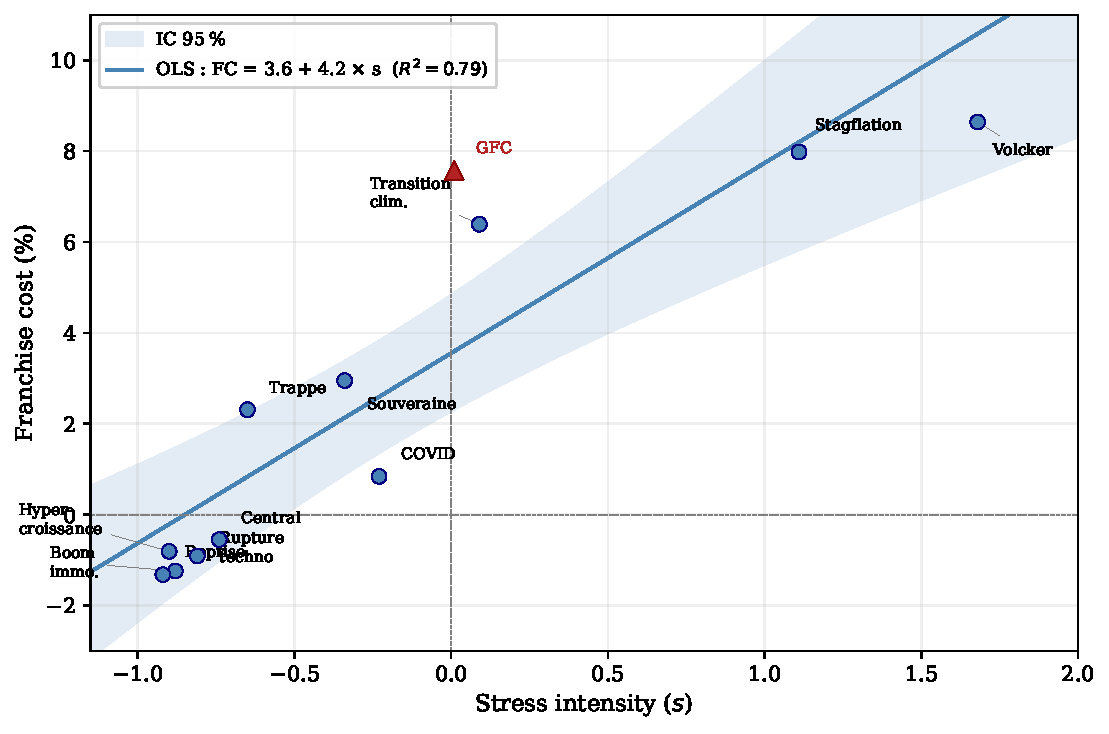
\includegraphics[width=0.85\textwidth]{fc_vs_stress.pdf}
\caption{Franchise cost vs stress intensity. Chaque point est un scénario. Droite OLS avec bande de confiance 95\,\%. La GFC (triangle rouge) est un outlier~: stress quasi-nul mais FC élevé.}
\label{fig:fc-scatter}
\end{figure}

\paragraph{Deux types de crises.} Le résidu GFC révèle une distinction structurelle entre deux mécanismes de création de valeur par l'optimiseur.

\emph{Crises diffuses} (Volcker, Stagflation, Transition climatique)~: le stress composite $s$ est élevé, toutes les classes souffrent proportionnellement au facteur systématique, et le FC observé est proche du FC prédit par l'OLS. L'optimiseur crée de la valeur parce que le stress agrégé est sévère et qu'il peut pivoter vers les classes à faible pondération (souverain, repos). Le modèle linéaire capture bien ce mécanisme.

\emph{Crises concentrées} (GFC, Souveraine)~: le stress agrégé est modéré ($s \approx 0$ pour la GFC), mais certaines classes s'effondrent (immobilier $-$29{,}5\,\%, dérivés $-$52{,}5\,\%) pendant que d'autres résistent (souverain $+$20{,}1\,\%). Le facteur unique sous-estime le FC parce qu'il ne capture pas la \emph{dispersion sectorielle} du choc. L'optimiseur crée de la valeur non pas parce que le stress est élevé, mais parce que l'hétérogénéité \emph{conjoncturelle} des rendements crée des arbitrages que l'allocation typique ne peut pas exploiter.

Le FC est donc piloté par deux canaux~: la sévérité macro (capturée par $s$, $R^2 = 0{,}79$) et la dispersion sectorielle (non capturée, responsable du résidu GFC). Un modèle multi-factoriel ou à signe classe-spécifique réduirait ce résidu --- c'est précisément l'objet de la Perspective~1 (section~\ref{sec:perspectives}, corrélations empiriques DCC-GARCH et conventions de signe classe-spécifiques).

\paragraph{Limites du calculateur.}
\begin{enumerate}[nosep]
  \item Le benchmark $\mathbf{w}_{\text{typ}}$ reflète déjà franchise et régulation~: on mesure la distance entre allocation contrainte et non contrainte, pas le coût de la franchise \emph{pure}.
  \item Le CIR optimal (20{,}6\,\%) est un artefact~: les coûts fixes (IT, compliance, réseau) ne sont pas réallouables proportionnellement aux poids. Le quantum du gain est une borne supérieure.
  \item $N = 12$ scénarios (10 degrés de liberté)~: $t = 6{,}09$ est significatif mais la puissance est limitée.
  \item Scénarios macro diffus uniquement~: un choc sectoriel ciblé stresserait les mêmes classes en typique et en optimal, réduisant le FC.
  \item Le coût réglementaire moyen est \emph{négatif} ($-$0{,}87\,\%)~: Phase~2 améliore le RAROC vs Phase~1 pure par régularisation (les contraintes empêchent la suroptimisation dans des classes à RAROC élevé mais volatile).
\end{enumerate}


\subsection*{Franchise cost sur le périmètre pe-bc}

Le même calculateur est appliqué au périmètre pe-bc (5~secteurs $\times$ 2~canaux, benchmark 97\,\% crédit / 3\,\% PE, 12~scénarios).

\begin{table}[htbp]
\centering
\caption{FC pe-bc~: scénarios de référence (Mds\texteuro, échelle 750~Mds RWA)}
\label{tab:fc-pebc-scenarios}
\small
\begin{tabular}{lrrrrrr}
\toprule
Scénario & RAROC$_{\text{typ}}$ & RAROC$_{\text{P1}}$ & RAROC$_{\text{opt}}$ & FC & RC & dEVA \\
\midrule
Central      & $+$1{,}61\,\% & $+$2{,}89\,\% & $+$1{,}32\,\% & $-$0{,}30 & $+$1{,}58 & $-$2{,}2 \\
GFC          & $-$0{,}67\,\% & $+$1{,}28\,\% & $-$0{,}67\,\% & $+$0{,}01 & $+$1{,}94 & $-$2{,}8 \\
Stagflation  & $-$5{,}96\,\% & $-$4{,}48\,\% & $-$6{,}35\,\% & $-$0{,}39 & $+$1{,}87 & $-$4{,}1 \\
Reprise      & $+$2{,}66\,\% & $+$6{,}11\,\% & $+$2{,}24\,\% & $-$0{,}42 & $+$3{,}88 & $-$1{,}8 \\
COVID        & $+$1{,}90\,\% & $+$4{,}28\,\% & $+$1{,}45\,\% & $-$0{,}45 & $+$2{,}83 & $-$1{,}9 \\
Boom immo.   & $+$2{,}81\,\% & $+$5{,}73\,\% & $+$2{,}24\,\% & $-$0{,}57 & $+$3{,}49 & $-$1{,}8 \\
\midrule
Moyenne (12 sc.) & --- & --- & --- & $-$1{,}95 & $+$2{,}83 & $-$2{,}4 \\
\bottomrule
\multicolumn{7}{l}{\footnotesize{FC $=$ RAROC$_{\text{opt}}$ $-$ RAROC$_{\text{typ}}$. RC $=$ coût régulatoire $=$ RAROC$_{\text{P1}}$ $-$ RAROC$_{\text{opt}}$. dEVA en Mds\texteuro.}} \\
\end{tabular}
\end{table}

\begin{table}[htbp]
\centering
\caption{Décomposition P\&L pe-bc en scénario Central (Mds\texteuro, 750~Mds RWA)}
\label{tab:fc-pebc-pnl}
\small
\begin{tabular}{lrrrr}
\toprule
Métrique & $w_{\text{typ}}$ & $w_{\text{P1}}$ & $w_{\text{opt}}$ & $\Delta$ Opt--Typ \\
\midrule
NII      & 10{,}2 & 16{,}7 &  8{,}6 & $-$1{,}6 \\
Pertes   &  8{,}8 & 12{,}1 & 10{,}2 & $+$1{,}4 \\
Profit   & $-$2{,}4 & $-$2{,}2 & $-$4{,}1 & $-$1{,}8 \\
Capital  & 98{,}2 & 127{,}0 & 101{,}5 & $+$3{,}4 \\
EVA      & $-$15{,}1 & $-$18{,}7 & $-$17{,}3 & $-$2{,}2 \\
\bottomrule
\end{tabular}
\end{table}

\paragraph{Régressions OLS pe-bc.}
Le modèle FC $= \alpha + \beta \times s$ donne $\beta = +0{,}10\,\%$ par unité de stress, avec $R^2 = 0{,}08$ et $t(\beta) = 0{,}95$ --- \textbf{non significatif}. Le FC pe-bc est indépendant du stress~: l'univers sectoriel est trop homogène pour qu'un choc macro crée une divergence exploitable. En revanche, le modèle dEVA $= \alpha + \beta \times s$ est très significatif ($\beta = -1{,}3$~Md, $R^2 = 0{,}83$, $t = -6{,}98^{***}$) mais de signe \textbf{négatif}~: l'optimiseur pe-bc fait pire en crise, car tous les secteurs de crédit sont corrélés et il n'existe aucun actif refuge.

\paragraph{Interprétation.}
Trois différences structurelles séparent les deux univers.
%
\begin{enumerate}[nosep]
  \item \textbf{Dimensionnalité et décorrélation.} En 14~classes, le souverain (RW $= 0\,\%$) et les repos (RSF $= 0\,\%$, collatéralisés) offrent des refuges décorrélés du crédit corporate. En pe-bc, les 5~secteurs partagent le même facteur $Z$ et des pondérations CRR3 similaires ($\sim$100\,\%). L'optimiseur n'a aucune marge de manœuvre.
  \item \textbf{Phase~2 inversée.} En 14~classes, la Phase~2 améliore le RAROC par régularisation (RC $= -$0{,}87\,\%). En pe-bc, elle le détruit (RC $= +$2{,}83\,\%), car satisfaire CET1/LCR/NSFR dans un univers 100\,\% crédit force la surpondération de l'immobilier --- le secteur au plus faible RAROC (1{,}50\,\%) mais au meilleur profil NSFR (duration 7~ans, RSF $= 0{,}85$).
  \item \textbf{Adaptation cyclique faible.} Le split PE sature au plafond de 8\,\% dans 10~scénarios sur~12 en pe-bc~: la contrainte CRR3 domine et les $\Delta w$ sectoriels ne varient que de quelques dixièmes de pourcent entre scénarios. En 14~classes, les $\Delta w$ varient de 1--2~pp entre scénarios (amplification en crise). L'adaptation significative au cycle nécessite une hétérogénéité structurelle des classes.
\end{enumerate}

\paragraph{Limites spécifiques au pe-bc.}
\begin{enumerate}[nosep]
  \item Le benchmark $\mathbf{w}_{\text{typ}}$ est construit (proportions sectorielles de SectorConfig, split 97/3 de la littérature BCE), pas observé sur une banque individuelle.
  \item Le CIR global (45\,\%) masque les différences opérationnelles (le crédit immobilier a un CIR plus élevé que le crédit technologie).
  \item La surpondération Immobilier par Phase~2 est un artefact des paramètres réglementaires (duration $= 7$~ans, RSF $= 0{,}85$)~; en pratique, l'immobilier commercial en crise est précisément ce que les régulateurs surveillent.
  \item La régression FC est non significative ($R^2 = 0{,}08$)~: le FC pe-bc est un ajustement structurel, pas un phénomène cyclique.
\end{enumerate}


\bibliographystyle{plainnat}
\bibliography{bibliographie}

\end{document}
